\documentclass[12pt,a4paper]{report}

\usepackage{styles/dolgozat}

\usepackage{listings}
\usepackage{styles/cpp}
\usepackage{styles/python}

\usepackage{hyperref}

\usepackage{amsmath}
\usepackage{diagbox}
\usepackage{wasysym}
\begin{document}

\pagestyle{empty} %a címlapon ne legyen semmi=empty, azaz nincs fejléc és lábléc

% A Miskolci Egyetem címere
{\large
\begin{center}
\vglue 1truecm
\textbf{\huge\textsc{Szakdolgozat}}\\
\vglue 1truecm

\includegraphics[width=4.8truecm, height=4truecm]{images/me_logo.png}\\
\textbf{\textsc{Miskolci Egyetem}}
\end{center}}

\vglue 1.5truecm %függõleges helykihagyás

% A szakdolgozat címe, akár több sorban is
{\LARGE
\begin{center}
\textbf{A drónokkal történő csomagszállítás adatkezelési problémáinak vizsgálata}
\end{center}}

\vspace*{2.5truecm}
% A hallgató neve, évfolyam, szak(ok), a konzulens(ek) neve
{\large
\begin{center}
\begin{tabular}{c}
\textbf{Készítette:}\\
Bajusz Máté Bence\\
Programtervező informatikus
\end{tabular}
\end{center}
\begin{center}
\begin{tabular}{c}
\textbf{Témavezető:}\\
Piller Imre
\end{tabular}
\end{center}}
\vfill
% Keltezés: Hely, év
{\large
\begin{center}
\textbf{\textsc{Miskolc, 2021}}
\end{center}}

\newpage


\newpage

\pagestyle{empty}

%Feladatkiiras
\begin{flushleft}
\textsc{\bfseries Miskolci Egyetem}\\
Gépészmérnöki és Informatikai Kar\\
Alkalmazott Matematikai Intézeti Tanszék\hspace*{4cm}\hfil \textbf{Szám:}
\end{flushleft}
\vskip 0.5cm
\begin{center}
\large\textsc{\bfseries Szakdolgozat Feladat}
\end{center}
\vskip 0.5cm
Bajusz Máté (BMA015) programtervező informatikus jelölt részére.\newline

\noindent\textbf{A szakdolgozat tárgyköre:} Adatmodellek, szimuláció, Go\newline

\noindent\textbf{A szakdolgozat címe:} \\
A drónokkal történő csomagszállítás adatkezelési problémáinak vizsgálata\newline

\noindent\textbf{A feladat részletezése:}

\medskip

\emph{A robotika fejlődésének és az online vásárlás egyre népszerűbbé válásának köszönhetően már kísérleti stádiumban vannak az olyan rendszerek, amelyek drónok segítségével oldják meg a csomagok kiszállítását. A dolgozat ezen problémakört vizsgálja az adatok továbbítása, kezelése és tárolása szempontjából.}

\medskip

\emph{Mivel ezen rendszerek még kialakulóban vannak, ezért a dolgozat szimulációk segítségével mutatja be, hogy az ilyen típusú logisztikai rendszerben hol keletkeznek adatok, azok milyen csatornákon kerülnek továbbításra és milyen mögöttes adatmodelleket lehet ezek perzisztens tárolásához használni. Elemzésre kerül a hibamentes és a sorrendhelyes adatátvitel kérdésköre, illetve a dolgozat összehasonlítja az elterjedt adatátviteli formátumokat.}

\medskip

\emph{A szimulációk Go programozási nyelven készülnek. Az adatmodellek vizsgálata esetében egyaránt bemutatásra kerülnek a relációs és a NoSQL adatmodellek és adatbáziskezelő rendszer implementációik.}

\vfill

\noindent\textbf{Témavezető:} Piller Imre (egyetemi tanársegéd) \newline

% \noindent\textbf{Konzulens(ek):} (akkor kötelezõ, ha a témavezetõ nem valamelyik matematikai tanszékrõl való; de persze lehet egyébként is)\newline

\noindent\textbf{A feladat kiadásának ideje:}2020. szeptember 28.\newline

%\noindent\textbf{A feladat beadásának határideje:}

\vskip 2cm

\hbox to \hsize{\hfil{\hbox to 6cm {\dotfill}\hbox to 1cm{}}}

\hbox to \hsize{\hfil\hbox to 3cm {szakfelelős}\hbox to 2cm{}}

\newpage

\vspace*{1cm}  
\begin{center}
\large\textsc{\bfseries Eredetiségi Nyilatkozat}
\end{center}
\vspace*{2cm}  

Alulírott \textbf{Bajusz Máté}; Neptun-kód: \texttt{BMA015} a Miskolci Egyetem Gépészmérnöki és Informatikai Karának végzős Programtervező informatikus szakos hallgatója ezennel büntetőjogi és fegyelmi felelősségem tudatában nyilatkozom és aláírásommal igazolom, hogy \textit{A drónokkal történő csomagszállítás adatkezelési problémáinak vizsgálata}
című szakdolgozatom saját, önálló munkám; az abban hivatkozott szakirodalom
felhasználása a forráskezelés szabályai szerint történt.\\

Tudomásul veszem, hogy szakdolgozat esetén plágiumnak számít:
\begin{itemize}
\item szószerinti idézet közlése idézőjel és hivatkozás megjelölése nélkül;
\item tartalmi idézet hivatkozás megjelölése nélkül;
\item más publikált gondolatainak saját gondolatként való feltüntetése.
\end{itemize}

Alulírott kijelentem, hogy a plágium fogalmát megismertem, és tudomásul veszem, hogy
plágium esetén szakdolgozatom visszautasításra kerül.

\vspace*{3cm}

\noindent Miskolc, \hbox to 2cm{\dotfill} .év \hbox to 2cm{\dotfill} .hó \hbox to 2cm{\dotfill} .nap

\vspace*{3cm}

\hspace*{8cm}\begin{tabular}{c}
\hbox to 6cm{\dotfill}\\
Hallgató
\end{tabular}



\newpage

\noindent 1.

\begin{tabular}{cl}
&szükséges (módosítás külön lapon) \\
A szakdolgozat feladat módosítása& \\
& nem szükséges\\
&\\
\hbox to 4cm{\dotfill}&\multicolumn{1}{c}{\hbox to 5cm{\dotfill}}\\
dátum& \multicolumn{1}{c}{témavezető(k)}
\end{tabular}
\vskip1.5mm

\noindent 2. A feladat kidolgozását ellenőriztem:

\vskip1.5mm

\begin{tabular}{l@{\hspace*{4cm}}l}
témavezető (dátum, aláírás):& konzulens (dátum, aláírás):\\
\dotfill&\dotfill\\
\dotfill&\dotfill\\
\dotfill&\dotfill
\end{tabular}

\vskip1.5mm

\noindent 3. A szakdolgozat beadható:

\vskip1.5mm

\begin{tabular}{@{\hspace*{1.3cm}}c@{\hspace*{2.1cm}}c}
\hbox to 4cm{\dotfill}&\multicolumn{1}{c}{\hbox to 5cm{\dotfill}}\\
dátum& \multicolumn{1}{c}{témavezető(k)}
\end{tabular}

\vskip1.5mm

\noindent 4.
\begin{tabular}[t]{@{}l@{\hspace*{1mm}}l@{\hspace*{1mm}}l@{}}
A szakdolgozat& \hbox to 3.5cm{\dotfill} &szövegoldalt\\
              & \hbox to 3.5cm{\dotfill} &program protokollt (listát, felhasználói leírást)\\
              &\hbox to 3.5cm{\dotfill}   &elektronikus adathordozót (részletezve)\\
              &\hbox to 3.5cm{\dotfill} & \\
              &\hbox to 3.5cm{\dotfill} &egyéb mellékletet (részletezve)\\
              &\hbox to 3.5cm{\dotfill} &\\
\end{tabular}
\newline tartalmaz.

\vskip1.5mm

\begin{tabular}{@{\hspace*{1.3cm}}c@{\hspace*{2.1cm}}c}
\hbox to 4cm{\dotfill}&\multicolumn{1}{c}{\hbox to 5cm{\dotfill}}\\
dátum& \multicolumn{1}{c}{témavezető(k)}
\end{tabular}

\noindent 5.

\begin{tabular}{ll}
&bocsátható\\
A szakdolgozat bírálatra& \\
& nem bocsátható\\
\end{tabular}

\vskip1.5mm

\noindent A bíráló neve: \hbox to 8cm{\dotfill}

\vskip4mm

\begin{tabular}{@{\hspace*{1.3cm}}c@{\hspace*{2.1cm}}c}
\hbox to 4cm{\dotfill}&\multicolumn{1}{c}{\hbox to 5cm{\dotfill}}\\
dátum& \multicolumn{1}{c}{szakfelelős}
\end{tabular}

\noindent 6.
\begin{tabular}[t]{@{}l@{\hspace*{1mm}}l@{\hspace*{1mm}}l@{}}
A szakdolgozat osztályzata& &\\
&a témavezető javaslata:& \hbox to 3cm{\dotfill}\\
&a bíráló javaslata:& \hbox to 3cm{\dotfill}\\
&a szakdolgozat végleges eredménye:& \hbox to 3cm{\dotfill}
\end{tabular}

\vspace*{4mm}

\noindent Miskolc, \hbox to 4.5cm{\dotfill} \hspace*{2.5cm}
\begin{tabular}[t]{cc}
\hbox to 6cm{\dotfill}\\
a Záróvizsga Bizottság Elnöke
\end{tabular}


\cleardoublepage
\pagenumbering{gobble}
\tableofcontents
\cleardoublepage
\pagenumbering{arabic}

\newpage

\pagestyle{fancy}

\Chapter{Bevezetés}

% A fejezet célja, hogy a feladatkiírásnál kicsit részletesebben bemutassa, hogy miről fog szólni a dolgozat.
% Érdemes azt részletezni benne, hogy milyen aktuális, érdekes és nehéz probléma megoldására vállalkozik a dolgozat.
\section{Probléma megfogalmazása}
Manapság a vásárlások egyre nagyobb része történik online, a termékeket pedig házhoz szállítják futárral.
A robotika fejlődése miatt, mint ahogy sok más egyszerű munka, a csomag szállítás is automatizálódni fog, melyre a drónok is bevethetők.
Egy ilyen rendszer nagyon sok adatot generál, amit fel kell dolgozni valós időben és eltárolni az adatokat.
Az elmúlt évtizedben olyan ekommersz óriások mint az Amazon már próbálkoztak több megoldással drón szállítás terén, így a közeljövőben elképzelhető, hogy egy nagyon valós probléma lesz a drónokat irányító, ellenőrző rendszer működtetése.

\Section{A szakdolgozat célja}
Egy olyan rendszert szeretnék bemutatni, ami gyors, hatékony, képes konkurrens működésre elosztott rendszerként a felhőben és valós időben tudja szimulálni a drónok működését, telemetria adatainak feldolgozását.
A rendszer több alkalmazásból épül fel, az alkalmazások Go (Golang) nyelven készültek és Docker konténerekben futnak.
A rendszer modulárisan épül fel, így különböző komponenseket kicserélhetjük, hogy összehasonlíthassuk a rendszer hatékonyságát a különböző konfigurációkkal.
Összehasonlításra kerül relációs és dokumentum alapú adatbázisok teljesítménye, valamint olyan internetes kommunikációra használt protokollok és formátumok hatékonysága mint a HTTP/2 gRPC, HTTP/1.1 JSON.
De olyan érdekességekről is lesz szó, hogy közlekedés szempontjából a Földön 2 pont között nem az egyenes a legrövidebb út.



% Ez egy egy-két oldalas leírás.
% Nem kellenek bele külön szakaszok (section-ök).
% Az irodalmi háttérbe, a probléma részleteibe csak a következő fejezetben kell belemenni.
% Itt az olvasó kedvét kell meghozni a dolgozat többi részéhez.

\Chapter{Koncepció}

\Section{Hasonló rendszerek, megoldások áttekintése}

Az Amazonnak már működő szállítási rendszere van, mely drónnal 30 percen belül eljuttatja az 2,3 kg-tól kevesebbet nyomó csomagokat az ügyfelekhez.
Ezek a drónok csak 24 km-es hatótávval rendelkeznek, így csak akkor biztonságos egy kézbesítés ha a célállomás maximum 12 km-re van.
A csomag maximum térfogatáról nincsenek pontos adatok.
Ezt a rendszert Prime Air-nek hívják \cite{prime-air}. Az Amazon Prime Air egy \aref{fig:prime} drónja.
\begin{figure}[h]
    \centering
    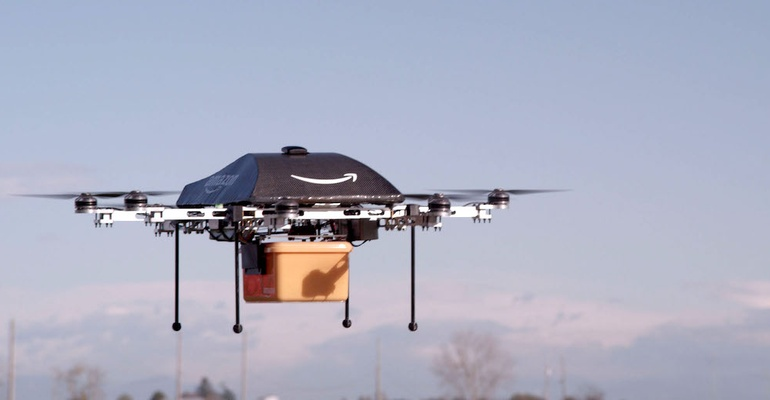
\includegraphics[scale=0.4]{images/prime.jpg}
    \caption{Amazon Prime Air drón}
    \label{fig:prime}
\end{figure}

Először 2016-ban próbálták ki, azóta még nem sikerült bevezetni különböző jogi korlátozások miatt. Olyan jogi elvárásoknak kell megfelelni, mint hogy:
\begin{itemize}
    \item Muszáj egy drón pilótának ellenőrizni a repülést és szükség esetén kötelező közbeavatkoznia.
    \item Egy ilyen pilóta csak 1 drónt felügyelhet egyszerre, kivéve ha rendelkezik megfelelő engedéllyel.
    \item A drónokat nem lehet közvetlen egy személy vagy gépjármű fellett működtetni.
    \item Problémát jelent továbba hogy nem minden légtér megfelelő a drónokkal való szállításra. A reptér mellett fekvő nagyvárosokban például biztos hogy nem lehet drónokkal szállítani.
    \item A csomagot szállító drónnak is kell rendelkeznie engedéllyel, hogy alkalmas kereskedelmi szállításra.
\end{itemize}

Az FAA 2020-ban engedélyezte az Amazonnak a drónokkal való csomagszállítást, de egyelőre csak tesztelik a technológiát pár városban.\\
Az Amazon felhőszolgáltásai között is található olyan szolgáltatás amellyel könnyedén kezelhetjük az IoT eszközöket, jelen esetben a drónokat.
Ilyen az IoT Core vagy az IoT Things Graph amin grafikus felületen összeköthetjük és beállíthatjuk az eszközeink közti kommunikációt. \\
A DHL is próbálkozott hasonló csomagkézbesítő megoldásokkal, ők egy úgynevezett  Parcelcopter-el \aref{fig:parcelcopter} szállították a csomagokat.

\begin{figure}[h]
    \centering
    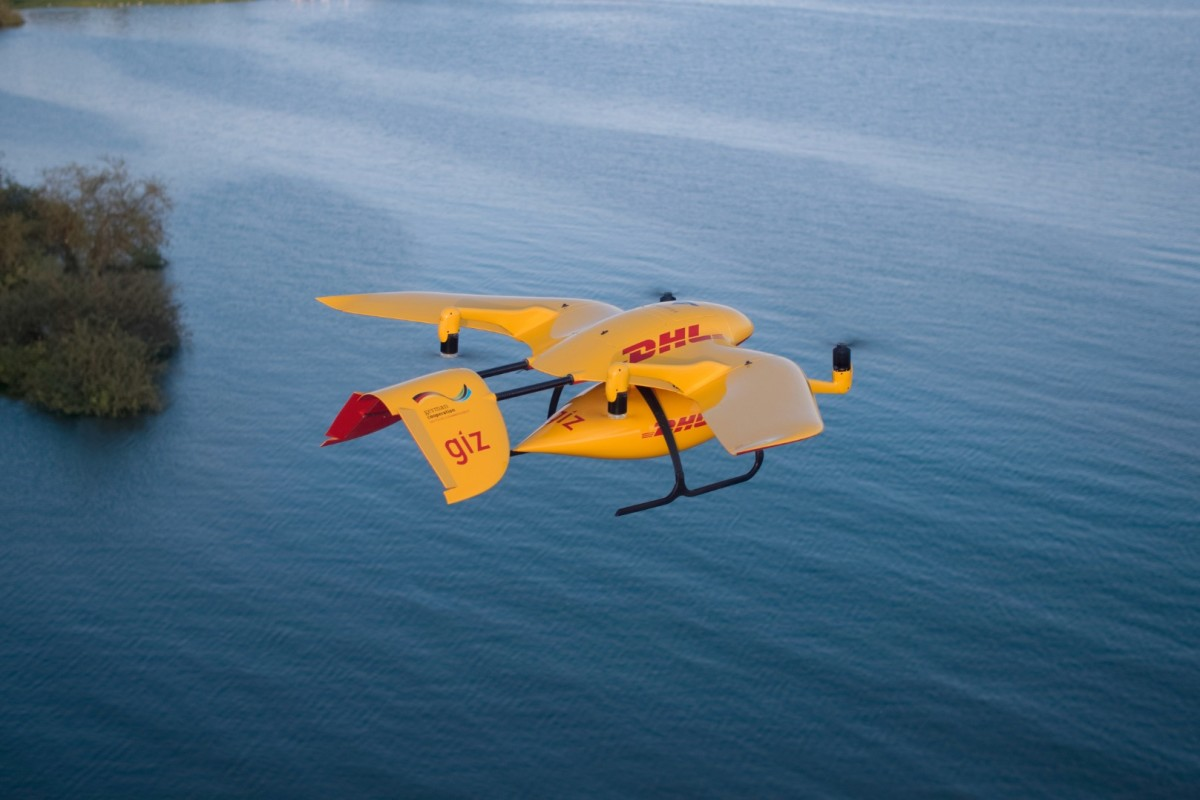
\includegraphics[scale=1.0]{images/parcelcopter.jpeg}
    \caption{DHL Parcelcopter V4.0}
    \label{fig:parcelcopter}
\end{figure}
Ám ők más problémát akarnak megoldani, a nagyon nehezen elérhető helyekre probálnak csomagokat szállítani.\\
A FlytBase \cite{flyt} vállalat már kínál szoftveres megoldásokat a automatizált drónok valós idejű figyelésére és irányítására, útvonal tervezésre valamint flotta menedzselésre.\\
A jövőben teljesen elképzelhető hogy a csomagok felét drónok szállítják ki. Csak az Amazon naponta átlagosan 7 millió csomagot szállít ki,
és bevallásuk szerint a csomagok 86\%-a drónnal szállítható.

\Section{A szállítási probléma absztrakt modellje}

A szállítási modellünk alapvetően úgy nézne ki, hogy a raktár és a kiszállítási hely közti távolság függvényében a csomagokat a raktárból drónok, vagy drónokkal felszerelt teherautók viszik ki.
A teherautók a kiszállítási hely közelében használnák a drónokat hogy kézbesítsék a drónokat.\\
A drónok 3G, 4G vagy 5G hálózaton kommunikálnának az adatközpontokkal.\\
Az adott hálózaton elérhető sávszélesség függvényében a drónok változtathatják az elküldött adatok mennyiségét és a küldés ütemezését, gyakoriságát.\\
A drónok repülése előre megtervezett, minél hatékonyabb kell hogy legyen de valós időben kell reagálniuk a helyzetekre, problémákra.\\
A drónokból a szállítás során keletkező nagymennyiségű adatot az adatközpontoknak valós időben hibamentesen
és hatékonyan kell tudnia kezelni anomáliák nélkül. Ehhez nagyon fontos a terhelés megfelelő elosztása. \\

A drónok csomag szállítási folyamatáról a következőket feltételezzük:
\begin{itemize}
    \item Egy drón  véges akkumlátoridővel vagy üzemanyaggal rendelkezik és mindig vissza kell tudnia térnie egy töltőállomásra, amely lehet egy drónszállító teherautó vagy raktár.
    \item A csomag kézbesítés a csomag átvételére vonatkozó ideje elhanyagolható.
    \item Minden drón fel van szerelve megfelelő kommunikácós és helymeghatározó eszközökkel, valamint az kommunikál az adatközpontokkal.
    \item Feltételezzük hogy a drónok el vannak látva szenzorokkal hogy felismerjék az akadályokat és erről értesítsék az adatközpontokat.
\end{itemize}
A mi esetünkben csak akkumlátorral üzemelő drónok lesznek. Minden drón küld telemetria adatokat,
ebbe benne lesz az akkumlátor töltöttség százalékban, valamint az akkumlátor hőmérséklete is.
A drónok a telemetria adatok részeként küldenek helymeghatérozásra alkalmas
földrajzi szélesség, hosszúság koordinátákat és magasságot.
Továbbá kapunk még információkat a drón sebességéről,
gyorsulásáról, tájoló iránytűjének állásáról, motorjainak hőmérsékletéről,
mindezt egy időpecséttel megbélyegezve hogy az üzenetek elküldésének idejét is tudjuk.

% TODO: Ezek így szövegesen leírva stimmelnek, de érdemes lenne jelöléseket is rakni hozzá, hogy fel lehessen majd írni az optimalizálási feladatot belőle.
\[
\begin{bmatrix}
    0.9 & 1 & 1 \\
    1 & 1.45 & 0.8\\
    1.32 & 1 & 0.8
\end{bmatrix}
\]

% TODO: Készíteni kellene egy sematikus ábrát, amin egy szállítási állapot, gráfos formában megadott probléma látható.

\Section{A Go nyelv áttekintése }

A Go program nyelv, (sokszor Golangként emlegetik) egy nyílt forráskódú modern programozási nyelv melyet a Google fejlesztett ki.\\
A Google-nél olyan problémák adódtak, hogy a konkurrenciát nem tudták megfelelően kezelni a még eredetileg
1 processzoros számítógépekre kifejlesztett nyelvek, mint a Java, C++.
Persze azóta sokat fejlődött ezen nyelvek konkurrenciakezelése de nem tudnak versenyezni a Go-val
ha a gépi és fejlesztői hatékonyságot is figyelembe vesszük.
Probléma volt az is, hogy ezeknek a nyelveknek nagyon nagy a fordítási idejük. A 2000-es évek végén ez azt jelentette
hogy egy Java vagy C++ program a Google-nél 1 hét alatt fordult le, csak hogy ki tudják próbálni.
A nyelvek bonyolultságával is baj volt, ahogy fejlődtek a nyelvek egyre nehezebb volt egy régi programot tovább fejleszteni,
illetve új programozóknak megtanulni a nyelvet.\\
Hogy ezeket a problémákat orvosolják, a Google a legjobb tervezőket hívta össze, hogy megalkossák a Go nyelvet.
A fejlesztést olyan szakemberek vezették, akik korábban a Unix operációs rendszer, a Java HotSpot JVM
vagy az UTF-8 karakterkódolás fejlesztésében is kulcsszerepet játszottak.
Például Ken Thompson, Rob Pike és Robert Griesemer.\\
A cél az volt, hogy régebbi általános célú nyelvek hiányosságait kiküszöböljék, és csökkentsék a bonyolultságot, hiszen a megváltozott üzleti és technológiai körülmények
között ezek a nyelvek nem bizonyultak elég hatékonynak.
Nem várhatták el hogy egy friss diplomás hatékonyan kezeljen egy olyan ''felpuffadt'' nyelvet mint a Java.\\
A felhőben való futtatásra olyan alkalmazások készítésére volt igény, amelyek nagy hatékonysággal futnak és kiválóan skálázódnak.
A végeredmény egy olyan nyelv amely általános célú, könnyen tanulható, kifejező, tömör, letisztult és hatékony.
Éppen ezért kiválóan alkalmazható ott, ahol a kódbázishoz nagyszámú, gyakran cserélődő, változó összetételű programozói gárda fér hozzá,
akár időben és földrajzi elhelyezkedésben is megosztva.\\
Szintaktikailag a C-hez hasonlít de nagyon könnyen tanulható nyelv.
A legnagyobb újítás a konkurrencia mechanizmus (főleg a saját ütemező) és hibakezelés volt.
A Go konkurrencia mechanizmusa megkönnyíti olyan programok írását amelyet a legtöbbet hozzák ki a többmagos és hálózaton összekötött gépekből.
Gyorsan lefordul gépi kódra de rendelkezik garbage collection-el és runtime reflection is van beépítve.
Gyors, statikus nyelv de úgy érezzük mintha egy dinamikus futás időben fordított nyelv lenne.
Tartalmaz \textit{race detector}-t is ami nagyon fontos egy ilyen nyelvben, mert fel tudja ismerni a konkurrens/párhuzamos programozásnál felmerülő gyakori problémákat.
Mivel nagyon jól kihasználja a gép erőforrásait és a hálózatot manapság a felhőben futó kódok nagyrésze Go.
Beszédes, hogy a Linux Foundation által létrehozott Cloud Native Computing Foundation (CNCF) keretein
belül támogatott projektek nagy része Go-ban íródott, többek között a Kubernetes, a Prometheus, az Istio, de ebben írták a Dockert is.\\

% TODO: Ide kellene hivatkozás.

\paragraph{A Go konkurrencia mechanizmusa} \mbox{} \\
A konkurrencia a nyelv alapjának része. A 3 legfontosab dolog ebből a szempontból az hogy a Go-nak saját ütemezője van,
a gorutinok (''goroutine'') és csatornák (''channel'').\\
A saját ütemező (scheduler) sokkal hatékonyabb mintha csak létrehoznánk egy processzt és hagynánk hogy az OS ütemezze,
mivel így az ütemező meg tudja határozni hogy az adott gorution milyen állapotban van (várakozik, futtatható, vagy fut) és hatékonyabban tudja
kiosztani az erőforrásokat. Értelemszerűen például egy blokkoló, épp I/O műveletet végző gorutint nem fog futtatni hanem helyette más gorutinokat részesít
előnyben. De fontos hogy az ütemező nem determinisztikus, így nem tudjuk előre megmondani melyik gorutin fog következni.\\
4 féle esemény fordulhat elő a Go programokban ami miatt az ütemező döntéseket hozhat:
\begin{itemize}
    \item A \emph{go} kulcsszó használata
    \item Garbage collection
    \item Rendszer hívások
    \item Szinkronizálás és orchesztráció, vezérelés
\end{itemize}
A \emph{go} kulcsszó használata: \par
A go kulcsszó létrehoz egy új gorutint, így az ütemezőnek lehetősége van beavatkozni.\\
Szinkronizálás és vezérlés: \par
Ha egy atomi, mutex, vagy csatorna művelet, függvényhívás miatt egy Gorutin blokkolni fog, az ütemező kontextus cserével egy másik gorutinnak adhat erőforrást. Ha a blokkolt Gorutin újra futtathatóvá válik, sorba állítja az ütemező és végül visszakapja az erőforrást.\\

A gorutinok ugyanabban a címtérben futnak, ezért a megosztott memóriához való hozzáférést szinkronizálni kell.
A csatornák a típusos vezetékek amelyeken adatokat küldhetünk és fogadhatunk a csatorna operátorral, <-.
Az adatok a nyíl irányába folynak.
\begin{python}
    ch <- v    // Snd v to channel ch.
    v := <-ch  // Receive from ch, and
    // assign value to v.
\end{python}
Alapértelmezett beaállítás szerint a csatornák blokkolnak amíg az egyik oldal küld vagy fogad.
Ez lehetővé teszi a szinkrinizációt anélkül hogy zárakat vagy feltétel változókat hoznánk létre.

Bufferelt csatornák
\begin{python}
    ch := make(chan int, 100)
\end{python}

\paragraph{A Go hibakezelése} \mbox{} \\
A hibakezelés nagyban megváltozott azzal hogy a Go-ban nem try és catch blokkba zárjuk a hibára futható programkódot
hanem van egy beépített hiba típus, ami a függvények visszatérési értéke lehet. Fontos tudni, hogy a Go-ban egy függvény többféle
visszatérési értékkel rendelkezhet. Amit mi írunk programkódot, szinte minden függvényünk utolsó visszatérési értéke egy hiba típus lesz.
Csak az olyan atomi műveleteket végző függvényeknél nem szoktunk hiba típust használni ami biztos hogy nem fut hibára normális körülmények között.
\begin{python}
    func Open(name string) (file *File, err error)
\end{python}
A fenti függvény például egy Fájl típus pointerét és egy hiba típust ad vissza. Ha nem futott hibába a program, az err változó nil értéket kap.

Tehát egy hiba kezelése például így nézhet ki:
\begin{python}
    file, err := Open(''fajlnev'')
    if err != nil {
    log.Println(err)
    return 0, err
    }
\end{python}



Pár vállalat aki használja:
\begin{itemize}
    \item Google
    \item Uber
    \item Netflix
    \item Youtube
    \item Dropbox
    \item BBC
\end{itemize}

Az előnyökhöz persze hátrányok is tartoznak, az egyszerűség mellé nem férnek el a generikus függvények.
Maga a nyelv nem tartalmaz osztályokat, illetve nincs öröklődés.
Viszont az objektum orientált paradigmákat használja és így is kell benne programozni.
Tartalmaz interfészeket, a típusokhoz így a structhoz is tudunk hozzárendelni úgynevezett receiver függvényeket, amelyeket más nyelvekben metódusoknak nevezünk, mert a típus egy példányára tudjuk meghívni.

% TODO: Külön szakaszban érdemes lenne kifejteni, hogy a konkurrencia kezelése (az aktor modell) pontosan mit takar, és hogy valósul meg a nyelvben.


\Chapter{Tervezés}

Itt kezdődik a dolgozat lényegi része, úgy értve, hogy a saját munka bemutatása.
Jellemzően ebben szerepelni szoktak blokkdiagramok, a program struktúrájával foglalkozó leírások.
Ehhez célszerű UML ábrákat (például osztály- és szekvenciadiagramokat) használni.

Amennyiben a dolgozat inkább kutatás jellegű, úgy itt lehet konkretizálni a kutatási módszertant, a kutatás tervezett lépéseit, az indoklást, hogy mit, miért és miért pont úgy érdemes csinálni, ahogyan az a későbbiekben majd részletezésre kerül.

Ebben a fejezetben az implementáció nem kell, hogy túl nagy szerepet kapjon.
Ez még csak a tervezési fázis.
(Nyilván ha olyan a téma, hogy magának az implementációnak a módjával foglalkozik, adott formális nyelvet mutat be, úgy a kódpéldákat már innen sem lehet kihagyni.)

\Section{Követelmények}

\subsection{Általános leírás}
Egy olyan elosztott rendszer környezetben működő szoftver létrehozása a cél, ami képes a drónszállítás közben keletkező valóságnak megfelelő adatokat szimulálni és hatékonyan feldolgozni.
Ezeknek az adatoknak a feldolgozását vizsgálom, több kontextusból.
Egyrészt a hálózaton való kommunikaáció hatékonyságát vizsgálom, tehát hogy mennyi adatforgalommal jár a kommunikáció,
és milyen hatékony ennek a kommunikációnak a feldolgozása, azaz a hálózaton használt formátum átalakítása a programban használt formátumra. Másrészt összehasonlítjuk az adatbázisba való mentés hatékonyságát.
Mivel elosztott rendszerekről van szó, nem egy darab program lesz.
Mikro-szervízként működnek majd a programok.
Ez azt jelenti, hogy ha 100 adat feldolgozást végző program fut egy terhelést elosztó proxy mögött, akkor ugyanolyan viselkedés várható mint ha csak 1 program futna.
A drón szenzorai által gyűjtött adatokat telemetria adatoknak nevezzük. A programok egy részének ezeket az adatokat kell tudnia generálni, egy másik részének feldolgoznia.

\subsection{Hatékonyság}
A hatékonyság alatt egyszerre értjük a teljesítményt, tehát hogy mennyire gyors a feldolgozás, és azt is hogy ez a feldolgozás mennyi erőforrást használ.
Célunk hogy a lehető legkevesebb adatforgalommal, a minimális CPU és memóriahasználattal de minél gyorsabban dolgozzuk fel az adatokat.


\subsection{Funkcionális követelmények}
A szimulációban több féle protokolt és adattovábbításra képes formátumot hasonlítunk össze, így a programot úgy kell felépíteni, hogy ki lehessen cserélni ezeket a végpontokat anélkül hogy a program üzleti logikájának működését befolyásolnánk.
Az adatközpontok és drónok közötti telemetria adat kommunikációt és annak feldolgozását összehasonlítjuk egy HTTP 1.1 -en műkodő JSON adatformátumot használó REST~\cite{Wikipedia-REST} API-n, egy HTTP 2 -n futó gRPC-t használó végponton is.
Az adatok mentését is több adatbázison kell tesztelni, így az adatbázisnak is cserélhetőnek kell lennie.

%TODO: ide még írni

\Section{Program struktúra}
\subsection{Architektúra, program felépítés}\label{subsec:architektúra-program-felépítés}
A probléma szimulációja 2 programból~\ref{fig:3program} áll. Egy program az adatközpont, egy program a drónok szerepét veszi fel, és van még egy egyszerű kliens ami,
paraméterek alapján konfigurálja a 2 program működését.
Az két program mikroszervízes struktúrában használhatónak kell lennie, hogy a valódi elosztott rendszeres működést megfelelően tudjuk tesztelni.\\
Az adatközpontot szimuláló program lesz a legbonyolultabb.
Ennek a programnak tudnia kell hibamentesen, adatvesztés nélkül feldolgozni és tárolnia az adatokat amiket a drónok küldenek, és vezérelni kell tudni a drónok indítását, logisztikai feladatait.

\begin{figure}[h]
    \centering
    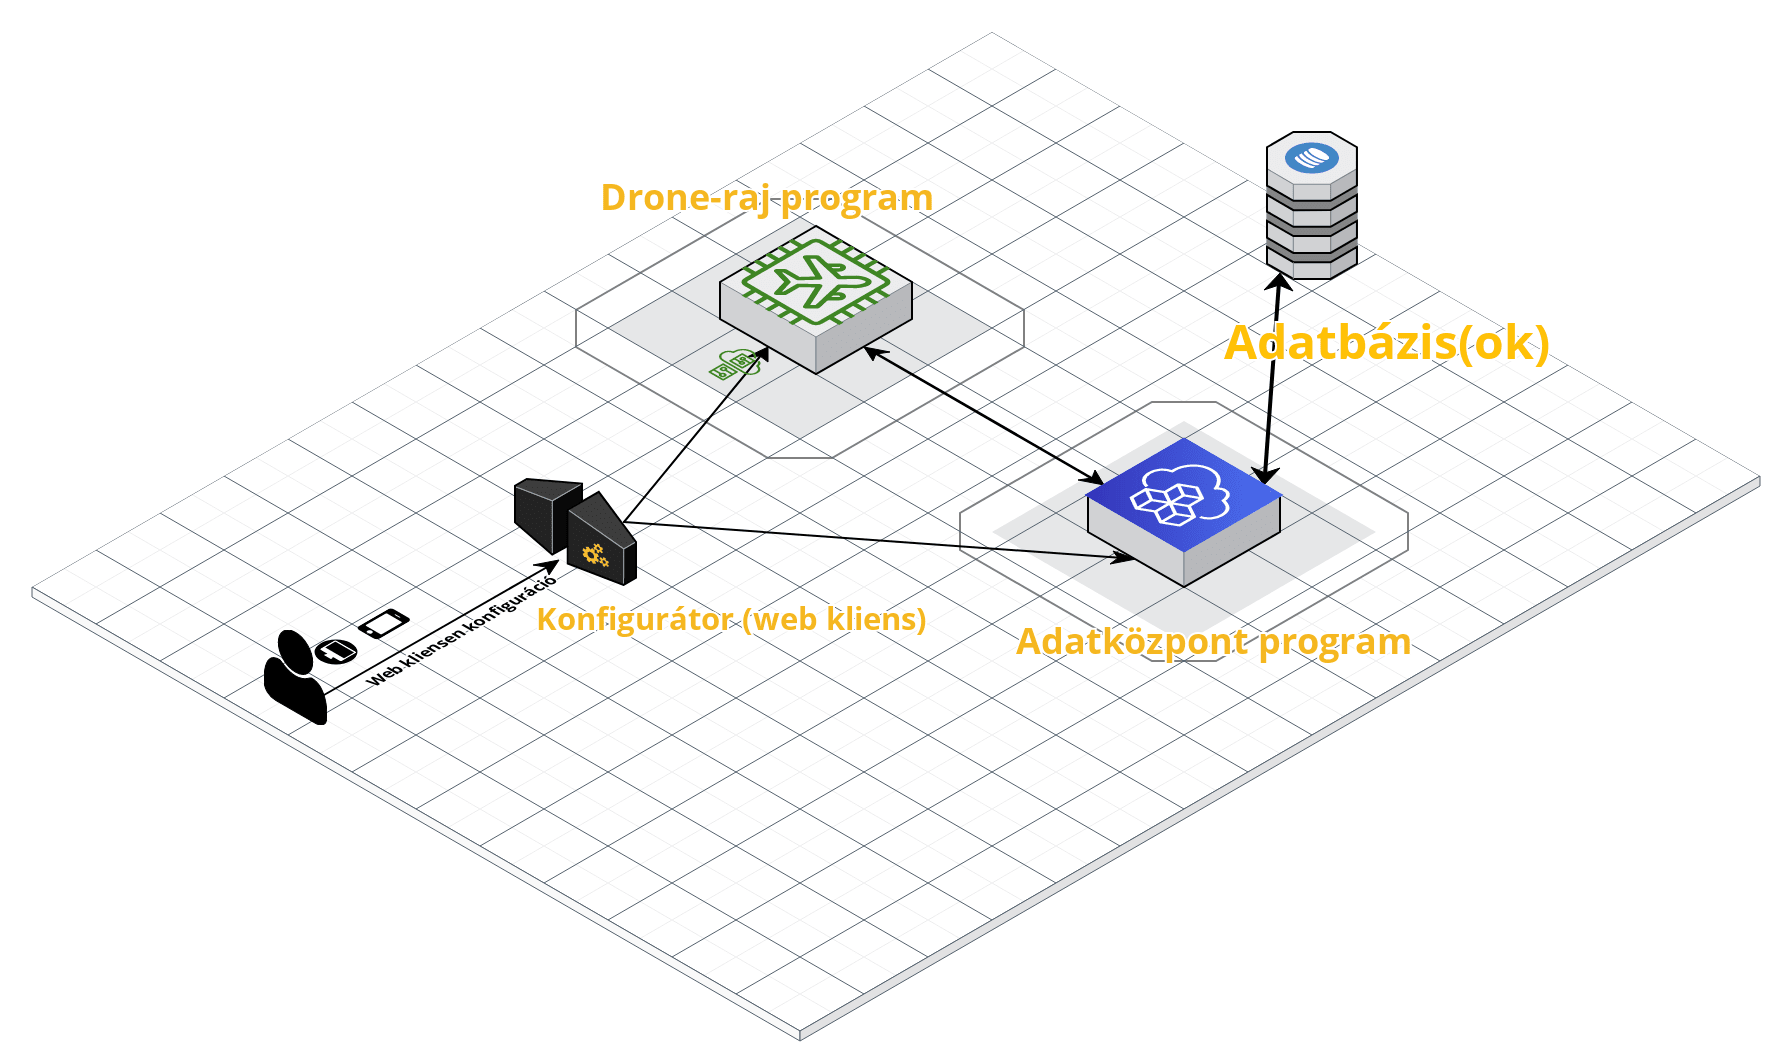
\includegraphics[scale=0.22]{images/szakdolgozat-3-program-abra.png}
    \caption{A 3 program}
    \label{fig:3program}
\end{figure}
Ahhoz hogy a programot a követelmányben megfogalmazott módon építsük fel, értem ez alatt azt hogy több protokollt és adatbázist hasonlítsunk össze egy olyan program architektúrát, felépítést kell választani ami megendegi ezt.
Erre a problémára megoldásként a Hexagonal architektúrát~\ref{fig:hexagonal-inward} és DDD tervezési alapelvet fogom alkalmazni.
\begin{figure}[h]
    \centering
    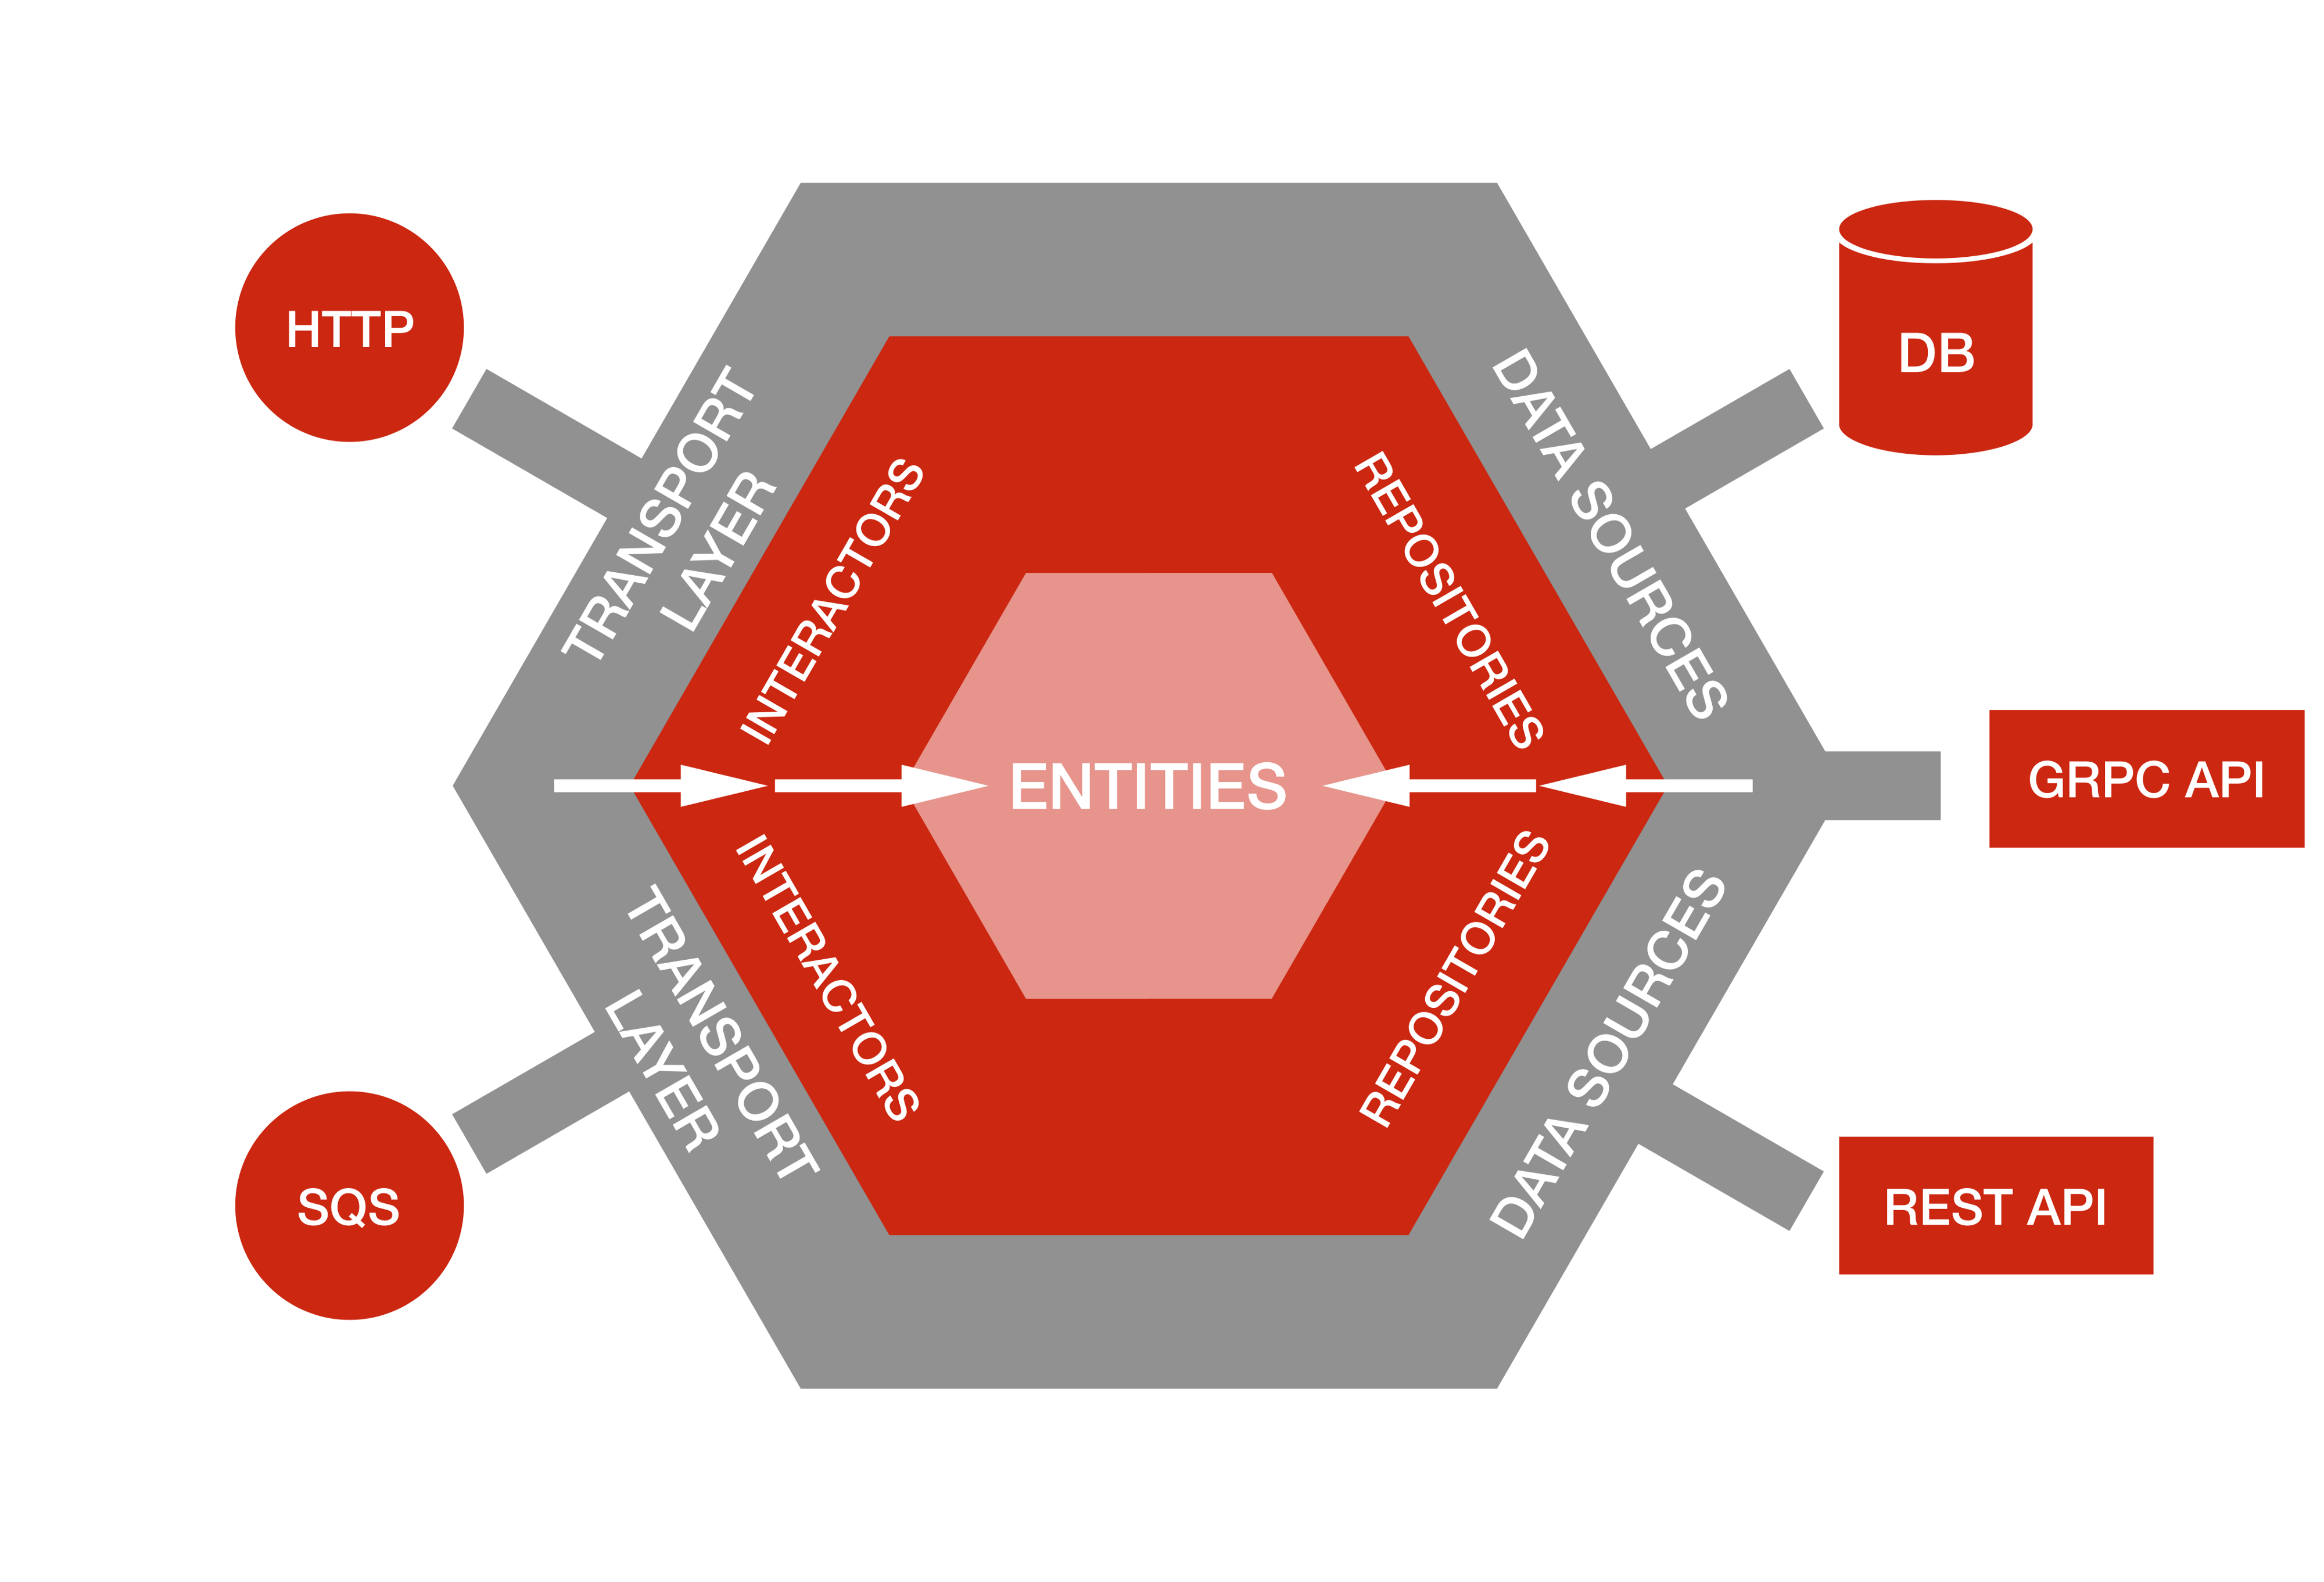
\includegraphics[scale=0.07]{images/hexa-inward.png}
    \caption{Hexagonal architecture inward pointing dependencies}
    \label{fig:hexagonal-inward}
\end{figure}
Így a program belülről kifelé rétegesen epül fel, interfaceket alkalmazva, úgy hogy a pontos implemetáció absztraktálva van, azaz csak az üzleti logikát ismerjük biztosan, minden ráépülő réteg implementációja cserélhető marad.
Minden réteg csak befelé mutat \ref{fig:hexagonal-inward}, így az üzleti logikánk megmaradhat, miközben az alkalmazás teljes infrastuktúráját kicserélhetnénk.
Így a végpontok ha teljesítik az interface elvárásait, csak dependency injection-el kicseréljük a végpontot és minden ugyanúgy működik, ám teljesen más az implementáció.
Azt hogy több fajta input és output végpontot hogy  támogatja az alkalmazás a következő ábra \ref{fig:hexagonal-inward} tökéletesen bemutatja.
Az alkalmazást fel lehet osztani verérlő és vezérelt részre. Ez nagyon jól igazodik az üzleti logikához, egy inputra szinte mindig valamiféle vezérlést várunk el,
tehát ahogz az alkalmazásunkat használjuk, vezéreljük akkor az adatok hatására valamit csináljon. Ezután az alkalmazásunk beszélhet más, külső forrásokkal, amiket az alkalmazás használ, azaz vezéreli őket.
Ilyen lehet egy adatbázis implementációja, vagy egy üzenet sor, amibe adatokat rakunk be, hogy valami más később kiolvassa.
Azért jó ez a felépítés, mert így például mindegy hogy a terminálból valamilyen konzolos applikáción keresztül hívjuk meg az alkalmazásunkat,
vagy egy webes felületről. A vezérelt egységeket is ki lehet cserélni, nem vagyunk röghöz kötve mert egyszer így lett megírva az alkalmazésunk, csak a megfelelő réteget kicseréljük, feltéve hogy megírtuk hozzá az implementációnkat és az implementációnk
az intefészen keresztül teljesít minden feltételt. Így például könnyen átállhatunk relációs adatbázisról egy dokumentum alapúra, vagy egy API-t is kicserélhetünk például JSON REST API-t gRPC-re ha valami miatt szükség van rá.
A Netflix is ezt az architektúrát használja \cite{netflix}, ugyanis a gyors növekedésük közben több skálázhatósággal összefüggő problémába ütköztek, amit úgy oldottak meg hogy
ebben az architektúrában\ref{fig:hexagonal-actor} szétosztották a feladatokat több, az adott kis feladatra megfelelő adatbázisra, mikroszervízre.
\begin{figure}[h]
    \centering
    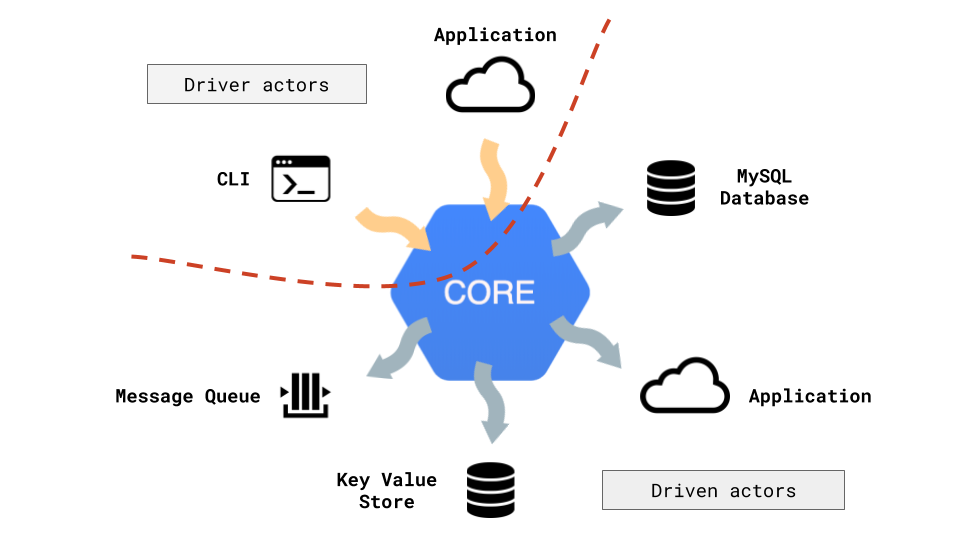
\includegraphics[scale=0.3]{images/hexa-actor.png}
    \caption{Hexagonal architecture ports and adapters}
    \label{fig:hexagonal-actor}
\end{figure}

\subsection{A Hexagonal architektúráról bővebben}\label{subsec:a-hexagonal-architektúráról-bővebben}
A hexagonal architektúra~\cite{hexagonal}, vagy másnéven portok és adapterek architektúra a szoftver tervezés során használt design.
Célja lazán összekapcsolt alkalmazás komponensek létrehozása, amelyek portok és adapterek segítségével könnyen összekapcsolhatóak.
Ez cserélhetővé teszi a program komponenseket bármilyen szinten, és megkönnyíti a teszteket.

Minden komponens nyitott egy "porton".
A komponensek közti kommunikáció ezeken a portokon történik egy adott protokoll alapján.
Ezt a protokollt a célnak megfelelően választjuk meg.
A portok és protokollok egy absztrak API-t definiálnak ami a megfelelő eszközzel implementálható\cite{hexagonal}.
A implementációt az adapterek valósítják meg, az objektum orientált nyelvekben interfész metódusokkal vannak összekötve a program magjával.
Ilyen lehet egy RPC hívás, webes szervíz, REST API, SQL lekérdezés.

\begin{figure}[h]
    \centering
    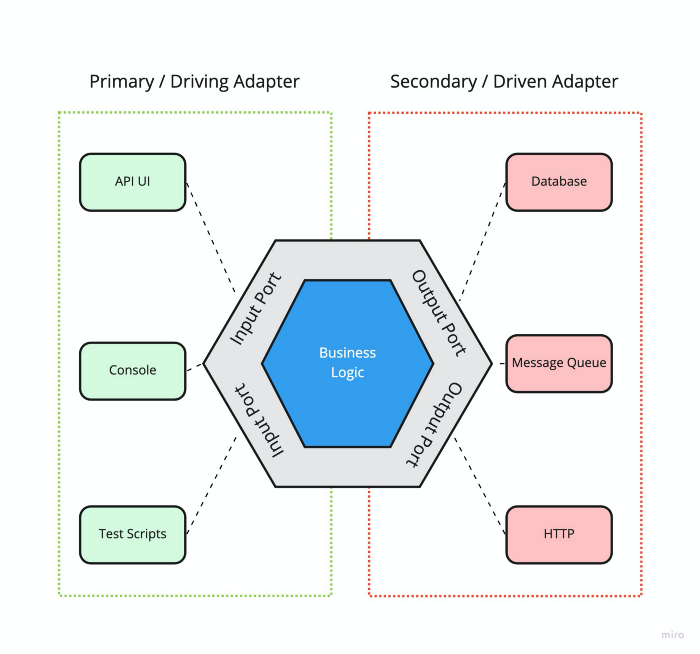
\includegraphics[scale=0.3]{images/ports-adapters}
    \caption{Hexagonal architecture driver and driven actors}
    \label{fig:hexagonal-ports-adapters}
\end{figure}

\subsection{REST architektúra}\label{subsec:rest-architektúra}

A REST (Representational State Transfer) \cite{Wikipedia-REST} egy szoftverarchitektúra típus internet alapú rendszerek számára.
Egy REST architektúrának meg kell felelni a következő megszorításoknak:
\begin{itemize}
    \item Kliens-szerver architektúra
    \item Állapotmentesség
    \item Gyorsítótárazhatóság
    \item Réteges felépítés
    \item Egységes interfész
\end{itemize}

\subsubsection{Kliens-szerver architektúra}
A kliensek el vannak különítve a szerverektől egy egységes interfész által. Az érdekeltségek ilyen nemű szétválasztása azt jelenti, például, hogy a kliensek nem foglalkoznak adattárolással, ami a szerver belső ügye marad, és így a kliens kód hordozhatósága megnő. A szerverek nem foglalkoznak a felhasználói felülettel vagy a kliens állapotával, így a szerverek egyszerűbbek és még skálázhatóbbak lehetnek. A szerverek és kliensek áthelyezhetőek és fejleszthetőek külön-külön is, egészen addig amíg az interfész nem változik meg.
\subsubsection{Állapotmentesség}
A kliens-szerver kommunikáció tovább korlátozott az által, hogy a szerveren nem tárolják a kliens állapotát a kérések között. Minden egyes kérés bármelyik klienstől tartalmazza az összes szükséges információt a kérés kiszolgálásához, és minden állapotot a kliens tárol. A szerver lehet állapottartó; ez a korlátozás csupán azt követeli meg, hogy a szerver oldali erőforrás-állapotok URL által címezhetőek legyenek. Ez nem csak a szerver felügyeletét teszi lehetővé, de megbízhatóbbá teszi őket a hálózati meghibásodásokkal szemben, valamint tovább fokozza a skálázhatóságot.
\subsubsection{Gyorsítótárazhatóság}
Mint ahogy a világhálón, a kliensek itt is képesek gyorsító-tárazni a válaszokat. A válaszoknak ezért impliciten vagy expliciten tartalmazniuk kell, hogy gyorsítótárazhatóak-e vagy sem. Így elkerülhető, hogy a kliens téves vagy elavult adatokat használjon fel újra. Egy jól menedzselt gyorsítótár lehetővé teszi, hogy teljesen megkerüljünk egyes kliens-szerver interakciókat, továbbá megnöveli a rendszer skálázhatóságát és a teljesítményét.
\subsubsection{Réteges felépítés}
Egy kliens általában nem tudja megmondani, hogy direkt csatlakozott-e a végpont szerverhez, vagy közvetítő segítségével. A közvetítő szerverek megnövelhetik a rendszer skálázhatóságát terheléseloszlás kiegyenlítéssel és megosztott gyorsítótárak használatával.
\subsubsection{Egységes interfész}
Az egységes interfész kliens és szerver között egyszerűsíti és kettéválasztja az architektúrát, és lehetővé teszi, hogy egymástól függetlenül fejlődjenek az egyes részek. Az interfész négy irányadó elve alább kerül részletezésre.


Ha ezeket a megkötéseket teljesíti a webes szolgáltatásunk, azt mondhatjuk hogy "RESTful".


\subsubsection{A REST működése}
A kliensek kéréseket indítanak a szerverek felé, a szerverek pedig feldolgozzák a kéréseket és egy választ küldenek vissza.
A kérések és a válaszok erőforrás reprezentációk köré épülnek.
Ezek az erőforrás reprezentációk a mi esetünkben JSON dokumentumok.
Az erőforrásokat az URL címével és a HTTP metódussal azonosítjuk.
A következő példában láthatjuk ahogy egy PUT metódussal és az URL-ben megadott paraméterrel pontosan tudjuk azonosítani mit szeretnénk.
A PUT requestet akkor használjuk ha egy már meglévő erőforrást szeretnénk felülírni, esetünkben az adatbázis konfigurációt kicseréljük.
A :name paraméter pedig megnevezi az erőforrást amire a meglévőt ki szeretnénk cserélni.
Válaszként egy JSON dokumentumot küldünk vissza válaszként a megfelelő státuszkóddal, hogy a kérés sikeres volt vagy sem.

\begin{python}
    router.PUT("/configure/database/:name", func(c echo.Context) error {
        switch c.Param("name") {
            case "mongodb":
            t.ChangeService(m)
            d.ChangeService(m)
            case "postgres":
            t.ChangeService(p)
            d.ChangeService(p)
            default:
            return echo.NewHTTPError(
            http.StatusBadRequest,
            "no such database supported"
            )
        }
        return c.JSON(http.StatusOK, "configuration complete")
    })
\end{python}


\subsection{HTTP/2 gRPC összehasonlítása HTTP/1.1 JSON üzenetváltással}

\paragraph{REST és HTTP 1.1, JSON üzenetváltás}
A mikroszevízes infrastuktúra egy nagyon elterjedt módja az elosztott rendszerek tervezésének.
Sok mikroszervíz a mai napig REST API-n kommunikál, HTTP 1.1-es protokollon keresztül és JSON dokumentumokat küldenek és fogadnak.
Ez a megoldás a fejlesztőknek kedvez, nagyon egyszerű így fejleszteni manapság, rengeteg eszköz van hogy megyorsítsa és megkönnyítse a munkánkat.
De ez a megoldás a teljesítmény rovására megy, ugyanis a következő problémák adódnak vele:
\begin{itemize}
    \item A HTTP/1.1  szöveg alapú és nagyon "nehéz". A kommunikáció hatalmas adatmennyiséget igényel, ez egy felesleges teher.
    \item A HTTP/1.1  állapotmentes, ezért az állapotokat csak a fejlécben tudjuk jelezni, ami nem tömörített.
    \item A HTTP/1.1  unáris - azaz - egy kérésre egy választ kapsz. Nem lehet egyszerre több kérdést küldeni, minden kérésre pontosan egy válasz jön.
    \item Minden egyes HTTP/1.1 kéréshez 3 irányú üzenet váltáshoz van szükség, csak hogy létrehozzuk a TCP kapcsolatot, mivel a TCP kapcsolat full duplex, és mindkét fél szinkronizálja és nyugtázza egymást.
\end{itemize}
Ebből arra következtetünk, hogy olyan szerver és szerver közötti kommunikációra ahol viszonylag sok apró kérés van, vagy a fenti problémák
akadályozzák a programunk működését, akkor érdemes más megoldások után néznünk.

\subsection{RPC}
Az RPC \cite{RPC} (Remote Procedure Call) egy szabvány, olyan távoli eljárás hívás amelynek segítségével használni lehet egy, ugyanabban a hálózatban található távoli gépen futó programot anélkül, hogy a hálózati részletekkel foglalkozni kellene.
Az RPC a kliens/szerver modellt használja (a kérő a kliens, a programot futtató fél a szerver).

\subsection{gRPC}
A gRPC \cite{gRPC} egy Google által fejlesztett RPC keretrendszer, főleg mikroszervizek közötti kommunikációra.
A gRPC HTTP/2-t használ és Protocol Buffert az üzenetváltáshoz JSON helyett. Ez szembemegy a megszokott mikroszervizes architektúra stílussal ami REST-re épül JSON üzenetváltásal HTTP/1.1-en.
Triviális, hogy a legfontosabb előnye az, hogy HTTP/2-n fut és az üzenetváltás Protocol Bufferekkel történik így sokkal gyorsabb és hatékonyabb.


\paragraph{HTTP/1.1 és HTTP/2 összehasonlítása}
A HTTP/2 egy sokkal hatékonyabb protokoll, a streameléssel elérhetjük azt, hogy az egyik fél több üzenetet is küld, a másik fél viszont csak a kérések legvégén válaszol.
\begin{table}[h]
    \centering
    \caption{HTTP/1.1 és HTTP/2}
    \label{tab:http}
    \begin{tabular}{|c|c|}
        \hline
        HTTP/1.1 & HTTP/2 \\
        \hline
        Szöveges formátum & Bináris formátum \\
        \hline
        Szöveges, nem tömörített fejléc & Tömörített fejléc \\
        \hline
        1 kérés, 1 válasz TCP kapcsolatonként & 1 TCP kapcsolatot újra felhasználunk,\\
        & Unáris kérések,\\
        & Szerver streamelés,\\
        & Kliens streamelés,\\
        & Két-irányú streamelés\\
        \hline
    \end{tabular}
\end{table}

\paragraph{Protocol Buffer és JSON összehasonlítása}

Beláthatjuk, hogy a Protocol Buffer adatforgalom kontextusban és hardveres erőforrás kontextusban is egy sokkal hatékonyabb eszköz üzenetek továbbítására mint a JSON, XML, stb hagyományos formátumok.
Mivel nem szöveges, lehet hogy nehezebb implementálni és debugolni a fejlesztőknek, viszont kevesebb adatforgalommal jár, és a számítógép erőforrásait is kíméli, nem úgy mint a JSON.

\begin{table}[h]
    \centering
    \caption{JSON és Protocol Buffer}
    \label{tab:message-exchange}
    \begin{tabular}{|c|c|}
        \hline
        JSON & Protocol Buffer \\
        \hline
        Nincs szigorú séma definíció & Szigorú séma formátum \\
        vagy típus & és típus biztonság \\
        \hline
        Szöveg alapú & Bináris \\
        \hline
        A szöveg formátum miatt lassú & Bináris formátum miatt gyors\\
        szérializáció és deszérializáció & szérializáció és deszérializáció\\
        CPU és memória intenzív & \\
        \hline
        Adatok manuális konvertálása & Generált kód a protokol buffer séma alapján\\
        \hline
    \end{tabular}
\end{table}

\newpage
\subsection{Adatbázisok}
Az adatok adatbázisba mentése, adatbázisból olvasása közben több probléma merülhet fel, a rendszer konkurrens felépítéséből kiindulva.
Például amikor az épp szabad drónoknak adunk feladatot, lehet hogy 2 vagy több egyede az adatközpont programunknak kiolvassa azt az értéket hogy
a drón nem csinál semmit, az állapota szabad, adhat neki feladatot ha van szállítsra váró csomag. De, az üzleti logika futtatása közben az egyik egyed módosíthatta
az értéket arra hogy már repül, vagy épp csomagot vesz fel. Az ilyen Lost Update problémákkal szemben védelmet ad, ha az adatbázis rendelkezik ACID tulajdonságokkal.
Az ACID tulajdonságok \ref{fig:acid} (atomiság, konzisztencia, izoláció, tartósság) felelősek az adatbázis integritásáért.

\begin{figure}[h]
    \centering
    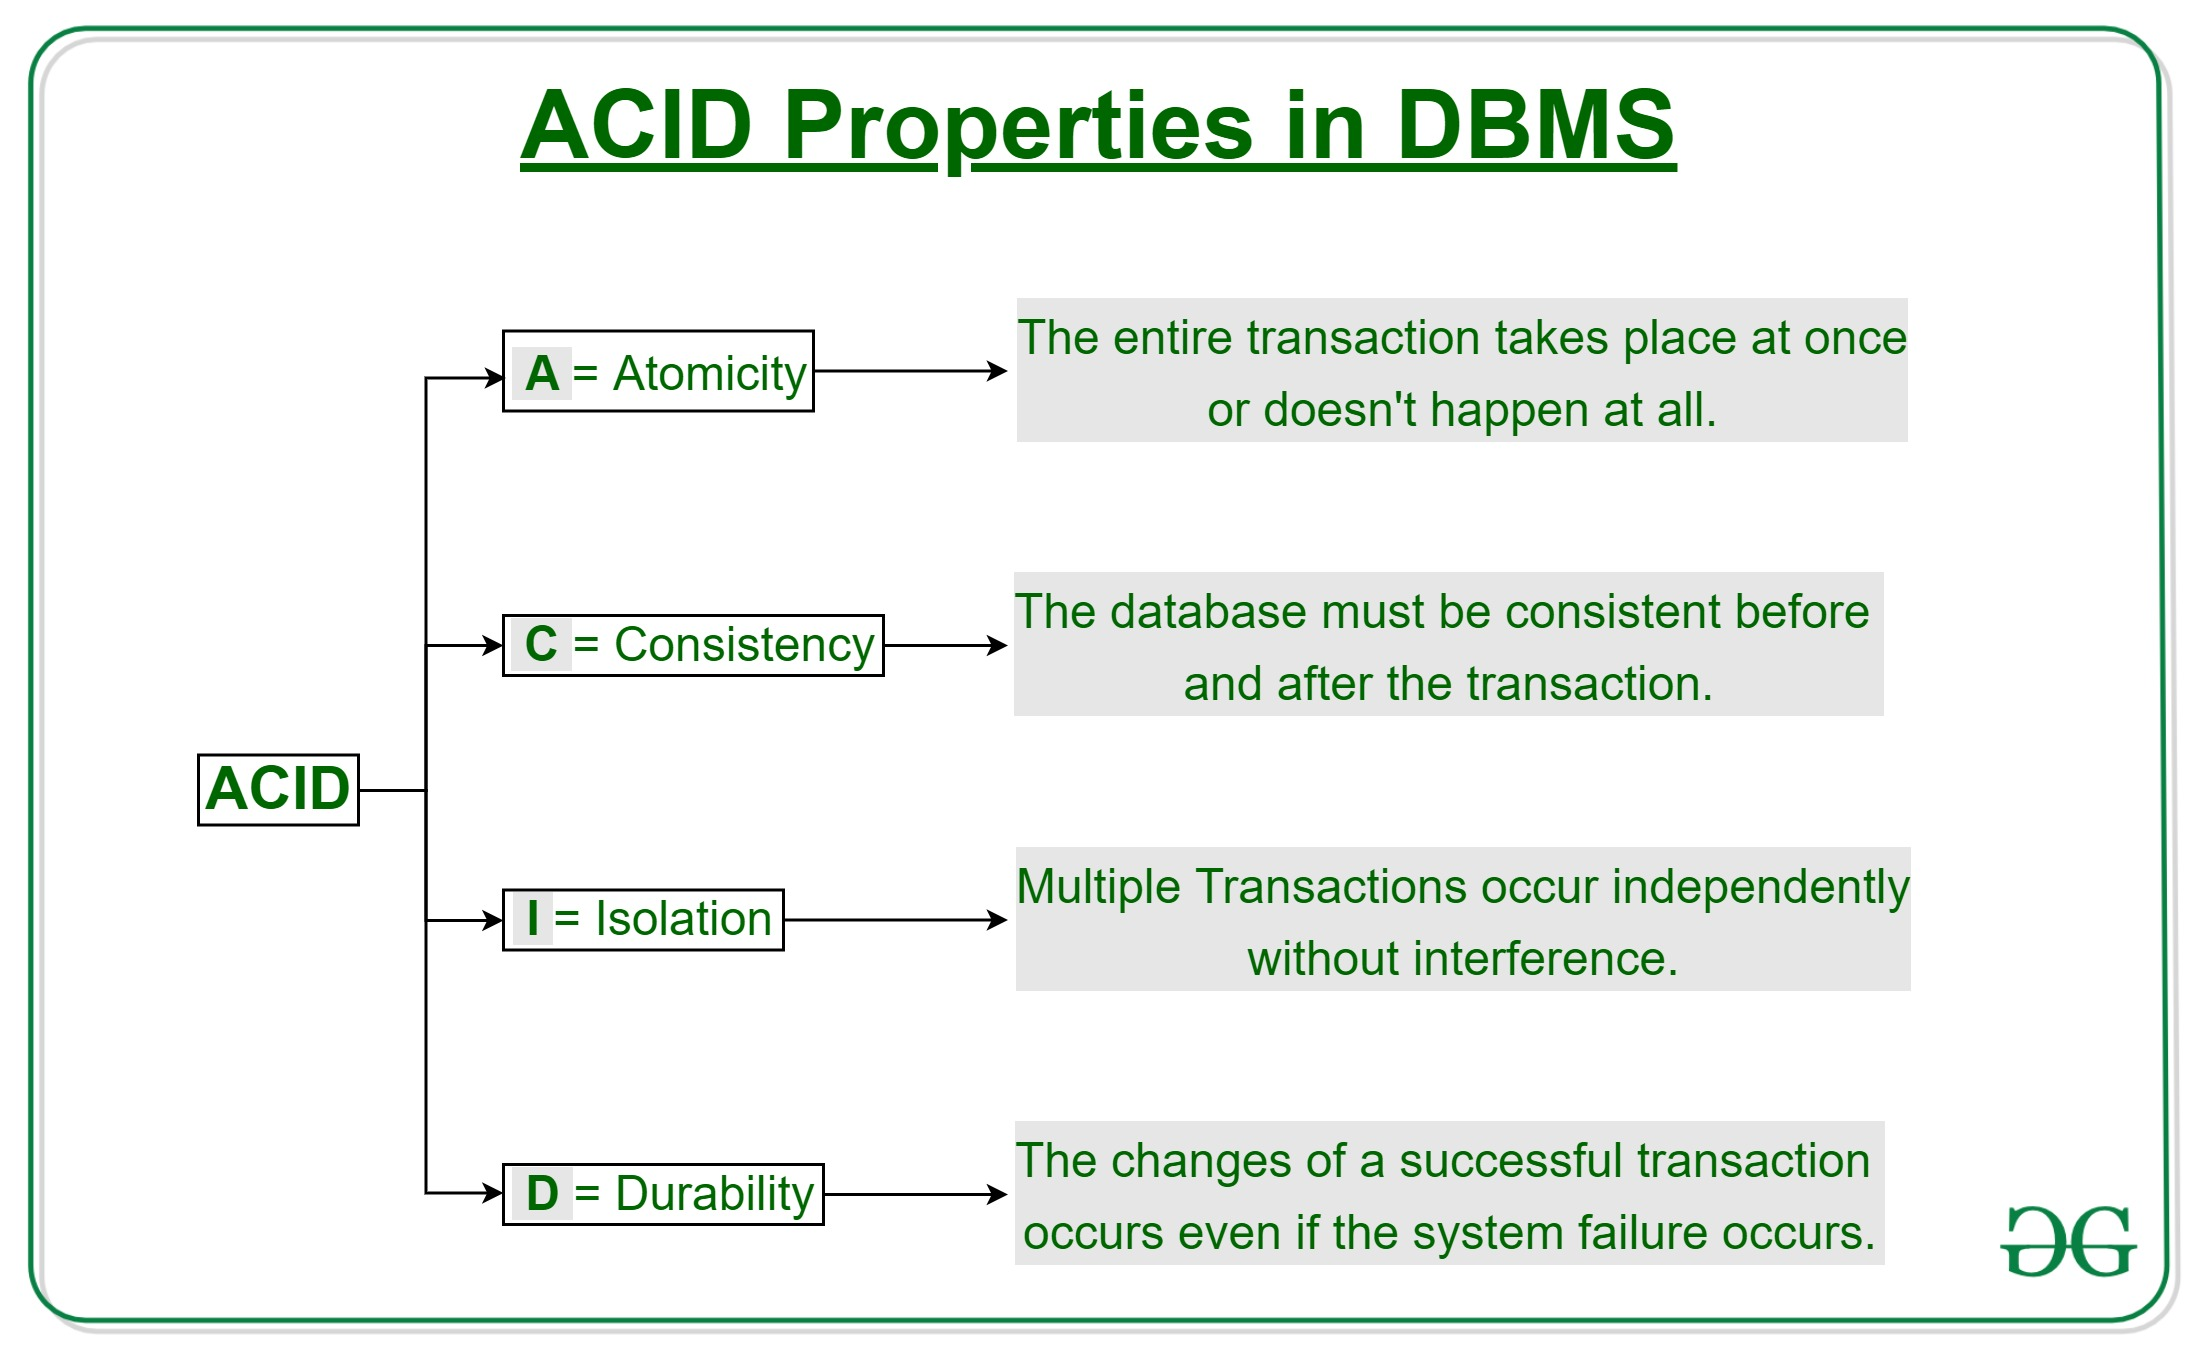
\includegraphics[scale=0.15]{images/ACID-Properties.jpg}
    \caption{ACID tulajdonságok}
    \label{fig:acid}
\end{figure}

Tehát csak olyan adatbázisok jöhetnek szóba a program implementálásánál aminek az integritása garantálható.
Hogy 2 eltérő adatbázist hasonlítsunk össze, egy SQL és egy NoSQL adatbázis ami teljesíti az ACID integritást megfelelő lesz.
A PostgreSQL adatbázis kíváló relációs adatbázis, nem véletlen, hogy az egyik legelterjedtebb. Teljesíti az ACID tulajdonságokat, és már 35 éve használják így biztosan megfelelően tesztelt.
A MongoDB dokumentum alapú adatbázis ACID, de csak dokumentum szintent. A mi szimulációnkhoz viszont így is megfelel a követelményeknek.
Érdekességként, a legtöbb dokumentum alapú adatbázis nem ACID, ezért nem annyira népszerűek.

\subsection{Protokollok és adatbázisok szerepe a programban}
A drón raj programot és az adatközpontot úgy tervezzük meg, hogy a telemetria adatok küldéséhez használt rész kicserélhető legyen valamilyen módon (például dependency injekción keresztül).
Így valósítjuk meg a több protokollon keresztüli kommunikációt. Az adatbázis végpontot is hasonlóan ki kell tudnunk cserélni, hogy ne kelljen módosítani a programon a különböző szimulációkhoz.
A következő kód példában láthatjuk, hogy működhet a dependency injekció. Itt a postgreSQL adatbázissal hoztuk létre a szervízt, de a mongoDB adatbázissal is létrehozhatjuk, ha teljesíti az interfész követelményeit.
\begin{python}
    postgresStorage, err := postgres.NewStorage(config.PostgresConfig)
    if err != nil {
        log.Println("Error connecting to database")
        panic(err)
    }
    mongoStorage, err := mongodb.NewStorage(config.MongoConfig)
    if err != nil {
        log.Println("Error connecting to database")
        panic(err)
    }
    var ts telemetry.Service
    var ds drone.Service
    var rs routing.Service
    ts = telemetry.NewService(postgresStorage, logger)
    rs = routing.NewService(logger)
    ds = drone.NewService(postgresStorage, jsonAdapter, logger, rs)
\end{python}

%TODO: ide még írni és a program struktúráját jobban megmutatni, a konkrét jegyzék struktúra is akár, hogy mi tartozik infrastruktúrához, mi a program magja stb. Interfacek kapcsolata,
%TODO: Új section ami a program folyamatával foglalkozik, nem a struktúrával
\Section{Szimuláció működésének folyamata}

A szimuláció működése azzal kezdődik, hogy elindítjuk az adatközpont programot.
Felcsatlakozik az adatbázisokra, majd létrehozza a szervizeket, és a REST API-n várja a bejövő kéréseket.
Ez lehet például egy konfigurációs kérés, a drónok lekérdezése, vagy a szállítás indítása.

Közben a drón-raj program is elindul, ez a program is egy REST API-n várja a kéréseket.
A drón raj program az API-n megkapja a drónokat és a hozzájuk rendelt csomagokat, majd megkezdódik a szimuláció, a drón-raj program telemetria adatokat küld az adatközpont programnak.
A drón-raj program olyan telemetria adatokat fog generálni, amelyek minél jobban a valsóságot tükrözik és ezeket az adatokat tovább fogja küldeni az adatközpontnak.
\begin{python}
{
    "telemetry": {
    "speed": 2,
    "location": {
    "latitude": 48.08092020178216,
    "longitude": 20.766208061642047
    },
    "altitude": 50,
    "bearing": 178.68412647009515,
    "acceleration": 0,
    "battery_level": 98,
    "motor_temperatures": [
    41,
    43
    ],
    "time_stamp": "2021-04-01T15:04:05.630Z",
    "drone_id": 2
    }
}
\end{python}

Ezeket a telemetria adatokat az adatközpont program fogadja a megadott porton és és lementi az adott adatbázisba. \ref{fig:adatkozpont-flow}

\begin{figure}[h]
    \centering
    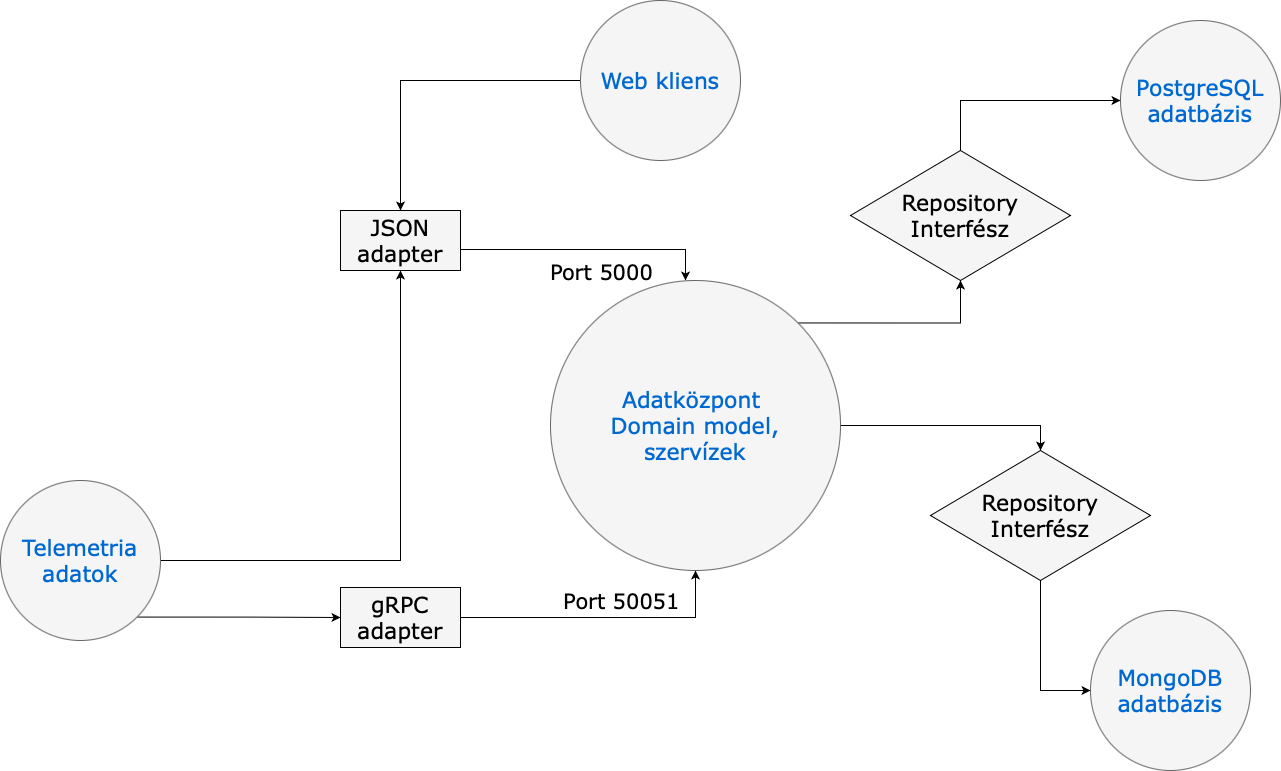
\includegraphics[scale=0.3]{images/adatkozpont-flow.png}
    \caption{Adatközpont program működésének folyamata}
    \label{fig:adatkozpont-flow}
\end{figure}


\Section{Táblázatok}

Táblázatokhoz a \texttt{table} környezetet ajánlott használni.
Erre egy minta \aref{tab:minta} táblázat.
A hivatkozáshoz az egyedi \texttt{label} értéke konvenció szerint \texttt{tab:} prefixszel kezdődik.

\begin{table}[h]
\centering
\caption{Minta táblázat. A táblázat felirata a táblázat felett kell legyen!}
\label{tab:minta}
\begin{tabular}{l|c|c|}
a & b & c \\
\hline
1 & 2 & 3 \\
4 & 5 & 6 \\
\hline
\end{tabular}
\end{table}

\Section{Ábrák}

Ábrákat a \texttt{figure} környezettel lehet használni.
A használatára egy példa \aref{fig:cimer}. ábrán látható.
Az \texttt{includegraphics} parancsba 
Az ábrák felirata az ábra alatt kell legyen.
Az ábrák hivatkozásához használt nevet konvenció szerint \texttt{fig:}-el célszerű kezdeni.

\begin{figure}[h]
\centering

\includegraphics[scale=0.3]{images/me_logo.png}
\caption{A Miskolci Egyetem címere.}
\label{fig:cimer}
\end{figure}

\Section{További környezetek}

A matematikai témájú dolgozatokban szükség lehet tételek és bizonyításaik megadására.
Ehhez szintén vannak készen elérhető környezetek.

\begin{definition}
Ez egy definíció
\end{definition}

\begin{lemma}
Ez egy lemma
\end{lemma}

\begin{theorem}
Ez egy tétel
\end{theorem}

\begin{proof}
Ez egy bizonyítás
\end{proof}

\begin{corollary}
Ez egy tétel
\end{corollary}

\begin{remark}
Ez egy megjegyzés
\end{remark}

\begin{example}
Ez egy példa
\end{example}


\Chapter{Szimuláció}


\section{Adatbázisok és modellek}
A programban a drón, és telemetria adatmodell a legfontosabb.
Ezeket az adatokat olvassuk és mentjük,illetve szükségesek az azonosításhoz vagy bármilyen értelmes következtetéshez a problémához kapcsolódóan.

\subsection{Modellek az adatközpont programban}
\subsubsection{Telemetria modell}
A programban a telemetria modell a következőképpen néz ki:

\begin{python}
    package models

    import "time"

    type Telemetry struct {
        Speed              float64          `json:"speed" db:"speed"`
        Location           GPS              `json:"location"`
        Altitude           float64          `json:"altitude"`
        Bearing            float64          `json:"bearing"
        Acceleration       float64          `json:"acceleration"`
        BatteryLevel       int              `json:"battery_level"`
        BatteryTemperature int              `json:"battery_temperature"`
        MotorTemperatures  []int            `json:"motor_temperatures"`
        Errors             []TelemetryError `json:"errors" db:"errors"`
        TimeStamp          time.Time        `json:"time_stamp"`
        DroneID            int              `json:"drone_id"`
    }

    type TelemetryError int

    const (
        MotorFailure TelemetryError = iota
        BeaconSignalStrengthLow
        BeaconSignalInterference
        BeaconTemperatureTooHigh
        GPSInt	eference
        GPSSignalLost
        GPSTemperatureTooHigh
        ProcessorTemperatureTooHigh
        BatteryFailure
        FailedToEjectPackage
        PackageLost
        DestinationDistanceTooFar
    )

    type GPS struct {
        Latitude  float64 `json:"latitude" bson:"latitude"`
        Longitude float64 `json:"longitude" bson:"longitude"`
    }

\end{python}


\subsubsection{Drón modell}
A DDD-ben leírt elvek alapján, a drón modell mindenféleképp egy Entity-nek felel meg.
\begin{python}
    type Drone struct {
        ID           int           `json:"id" db:"drone_id" bson:"id"`
        Telemetry    Telemetry     `json:"telemetry" bson:"telemetry"`
        Parcel       Parcel        `json:"parcel"`
        Destinations []Destination `json:"destinations"`
        Consumption  float64       `json:"consumption"`
        Weight       float64       `json:"weight"`
        State        DroneState    `db:"state" bson:"state"`
    }

    type DroneState string

    const (
    DroneFree     DroneState = "free"
    DroneInFlight DroneState = "in-flight"
    )
\end{python}


\subsubsection{Parcel modell (szállítandó csomag)}
A drónok által szállított csomag így néz ki:
\begin{python}
    type Parcel struct {
        ID            int             `json:"id" db:"id" bson:"id"`
        TrackingID    string          `json:"tracking_id" `
        Name          string          `json:"name" db:"name" bson:"name"`
        Weight        float64         `json:"weight" db:"weight"`
        Location      GPS             `json:"location" bson:"location"`
        FromAddress   ShippingAddress `json:"from_address"`
        ToAddress     ShippingAddress `json:"to_address"`
        DropOffSite   GPS             `bson:"drop_off_site" `
        AssignedDrone int             `json:"assigned_drone" `
    }
\end{python}

\subsection{Relációs adatbázis, PostgreSQL}
A relációs adatbázissal is működik a szimuláció.
\paragraph{Relációs modell \ref{fig:postgres} } \mbox{} \\

\begin{figure}[h]
    \centering
    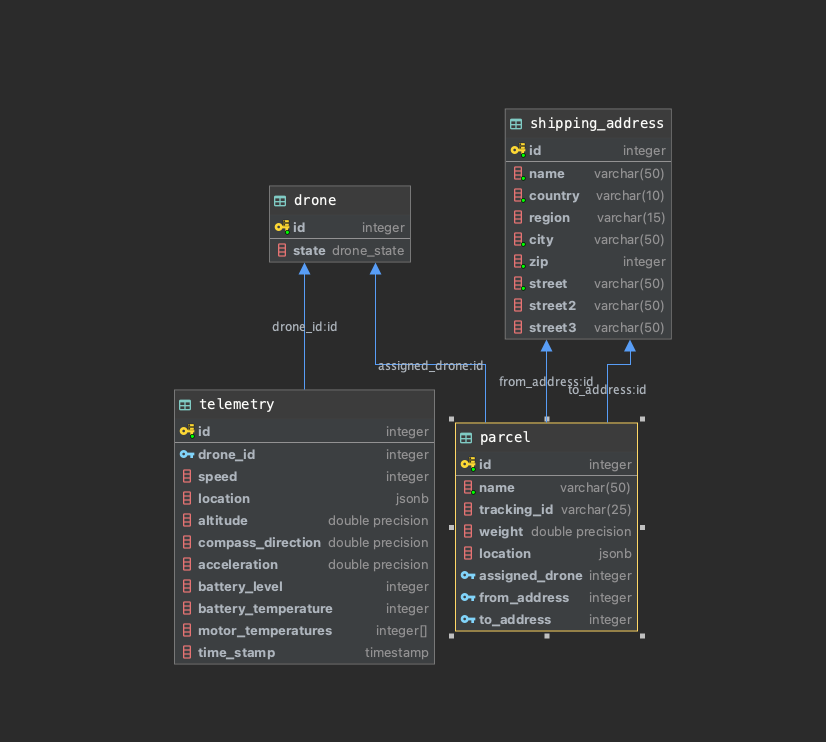
\includegraphics[scale=0.4]{images/postgres.png}
    \caption{PostgreSQL adatbázis modell}
    \label{fig:postgres}
\end{figure}

%TODO: Esetleg Er model


\subsubsection{Lost Update probléma}
A legtöbb relációs adatbázis támogatja a tranzakciókat. A tranzakciók ACID tulajdonságokkal bírnak.
Adatbázisok esetén az ACID az Atomicity (atomiság), Consistency (konzisztencia), Isolation (izoláció), és Durability (tartósság) rövidítése. Ezek nélkül az adatbázis integritása nem garantálható.
A PostgreSQL többféle izolációs szintet biztosít a tranzakciókhoz \cite{postgresql}. A Lost Update problémát garantáltan megoldja a PostgreSQL `Serializable` izolációs szintje.
\begin{table}[h]
    \centering
    \caption{ Standard SQL Transaction Isolation Levels}
    \begin{tabular}{l|c|c|c|}
Isolation Level & Dirty Read  & Nonrepeatable Read & Phantom Read\\
        \hline
Read uncommitted  & Possible & Possible & Possible \\
\hline
Read committed & Not possible & Possible & Possible \\
\hline
Repeatable read & Not possible & Not possible & Possible \\
\hline
Serializable & Not possible & Not possible & Not Possible \\
        \hline
    \end{tabular}
\end{table}

\subsubsection{PostgreSQL telepítése az alkalmazáshoz}\label{subsubsec:postgresql-telepítése-a-programhoz}

Ha nem található a fejlesztői környezetünkben PostgreSQL adatbázis, akkor \href{https://www.postgresql.org/download/}{telepíteni kell azt}.
Az adatbáziskezelőhöz csatlakozva, le kell futtatni a következő SQL scriptet.

\begin{lstlisting}[language=sql]
    CREATE TYPE drone_state AS ENUM ('free', 'in-flight');
    CREATE TABLE drone
    (
    id          SERIAL PRIMARY KEY,
    state       drone_state      DEFAULT 'free',
    weight      DOUBLE PRECISION default 4,
    consumption DOUBLE PRECISION DEFAULT 500
    );

    CREATE TABLE warehouse
    (
    id  SERIAL PRIMARY KEY,
    location_latitude DOUBLE PRECISION DEFAULT 48.080922,
    location_longitude DOUBLE PRECISION DEFAULT 20.766208
    );

    CREATE TABLE shipping_address
    (
    id      SERIAL PRIMARY KEY,
    name    VARCHAR(50) NOT NULL,
    country VARCHAR(10) NOT NULL,
    region  VARCHAR(15) DEFAULT NULL,
    city    VARCHAR(50) NOT NULL,
    zip     INT         NOT NULL,
    street  VARCHAR(50) NOT NULL,
    street2 VARCHAR(50) DEFAULT NULL,
    street3 VARCHAR(50) DEFAULT NULL
    );

    CREATE TABLE parcel
    (
    id                 SERIAL PRIMARY KEY,
    name               VARCHAR(50) NOT NULL,
    tracking_id        VARCHAR(25)               default '',
    weight             DOUBLE PRECISION          default 1,
    drop_off_latitude  DOUBLE PRECISION          DEFAULT 0,
    drop_off_longitude DOUBLE PRECISION          DEFAULT 0,
    assigned_drone     INT REFERENCES drone (id) DEFAULT NULL,
    from_address       INT REFERENCES shipping_address (id),
    to_address         INT REFERENCES shipping_address (id)
    );

    CREATE TABLE telemetry
    (
    id                  SERIAL PRIMARY KEY,
    drone_id            INT REFERENCES drone (id),
    speed               DOUBLE PRECISION DEFAULT 0,
    latitude            DOUBLE PRECISION DEFAULT 0,
    longitude           DOUBLE PRECISION DEFAULT 0,
    altitude            DOUBLE PRECISION default 1,
    bearing             DOUBLE PRECISION DEFAULT 0,
    acceleration        DOUBLE PRECISION DEFAULT 0,
    battery_level       INT              DEFAULT NULL,
    battery_temperature INT              DEFAULT NULL,
    motor_temperatures  INTEGER[],
    errors              INTEGER[],
    time_stamp          timestamp        DEFAULT NULL
    );
    INSERT INTO warehouse (id) VALUES (1);
\end{lstlisting}


\subsection{Dokumentum alapú adatbázis, MongoDB}

\subsubsection{Vizualizáció}

\begin{figure}[hbt!]
    \centering
    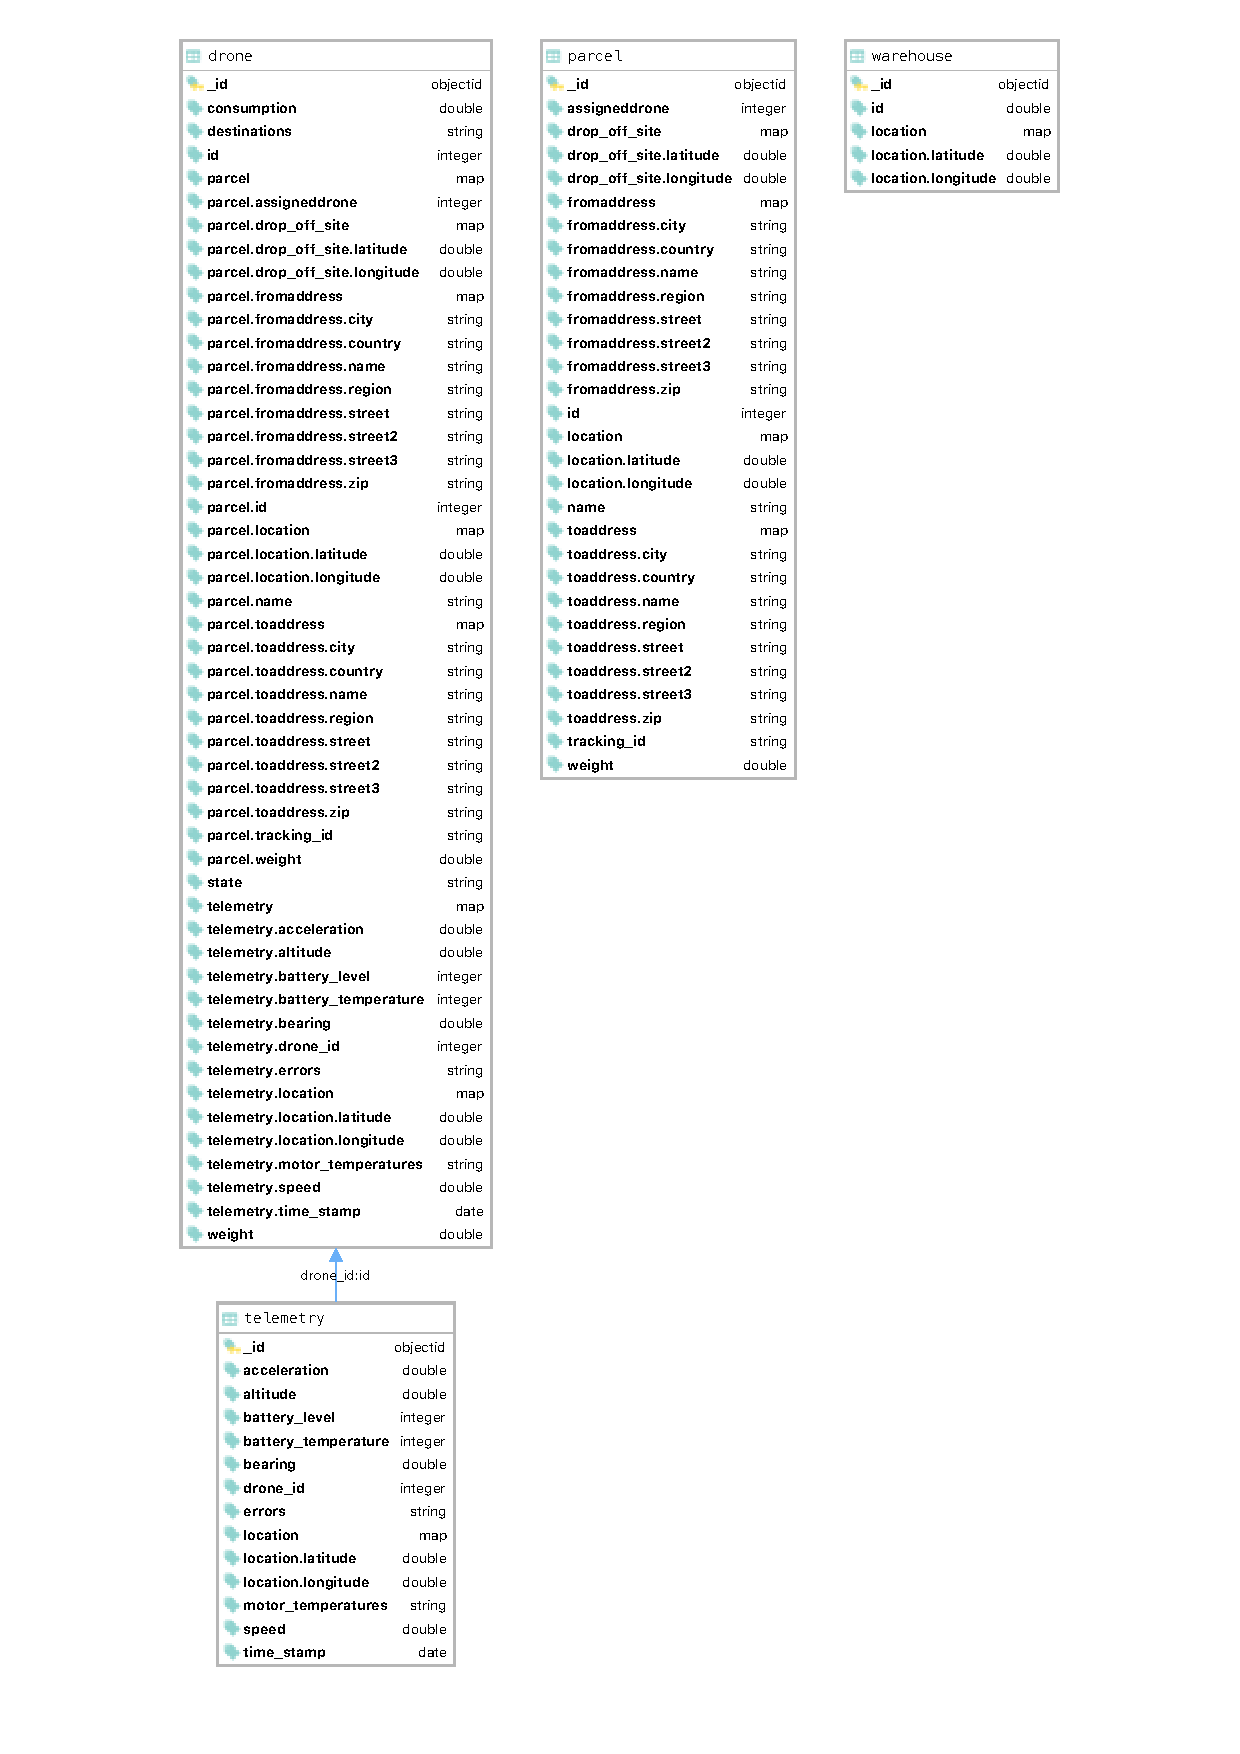
\includegraphics[scale=0.7]{images/mongo.pdf}
    \caption{MongoDB adatbázis vizualizáció}
    \label{fig:mongodb}
\end{figure}

\subsubsection{MongoDB telepítése az alkalmazáshoz}\label{subsubsec:mongodb-telepítése-az-alkalmazáshoz}
Ha nem található a fejlesztői környezetünkben MongoDB adatbázis, akkor \href{https://www.mongodb.com/try/download/community}{telepíteni kell azt}.
Az adatbáziskezelő konzolján keresztül le kell futtatni a következő két parancsot, egy megfelelő jogosultságú felhasználóval.
Ez egyik parancs létrehozza a drone\_delivery adatbázist, a másik parancs létrehoz nekünk egy felhasználót az előbb létrehozott adatbázishoz.
A későbbiekben ezzel a felhasználóval csatlakozunk az adatbázishoz.

\begin{python}
    use drone_delivery
\end{python}

\begin{python}

    db.createUser(
        {
        user: "drone-user",
        pwd: "drone-pwd",
        roles: [
            {
            role: "readWrite",
            db: "drone_delivery"
        }
        ]
    }
    )
\end{python}

\Section{Szimuláció működésének folyamata}

A szimuláció működése azzal kezdődik, hogy elindítjuk az adatközpont programot.
Felcsatlakozik az adatbázisokra, majd létrehozza a szervizeket, és a REST API-n várja a bejövő kéréseket.
Ez lehet például egy konfigurációs kérés, a drónok lekérdezése, vagy a szállítás indítása.

Közben a drón-raj program is elindul, ez a program is egy REST API-n várja a kéréseket.
A drón raj program az API-n megkapja a drónokat és a hozzájuk rendelt csomagokat, majd megkezdódik a szimuláció, a drón-raj program telemetria adatokat küld az adatközpont programnak.
A drón-raj program olyan telemetria adatokat fog generálni, amelyek minél jobban a valsóságot tükrözik és ezeket az adatokat tovább fogja küldeni az adatközpontnak.
\begin{python}
{
    "telemetry": {
    "speed": 2,
    "location": {
        "latitude": 48.08092020178216,
        "longitude": 20.766208061642047
    },
    "altitude": 50,
    "bearing": 178.68412647009515,
    "acceleration": 0,
    "battery_level": 98,
    "motor_temperatures": [
    41,
    43
    ],
    "time_stamp": "2021-04-01T15:04:05.630Z",
    "drone_id": 2
}
}
\end{python}

Ezeket a telemetria adatokat az adatközpont program fogadja a megadott porton és lementi az adott adatbázisba. \ref{fig:adatkozpont-flow}

\begin{figure}[h]
    \centering
    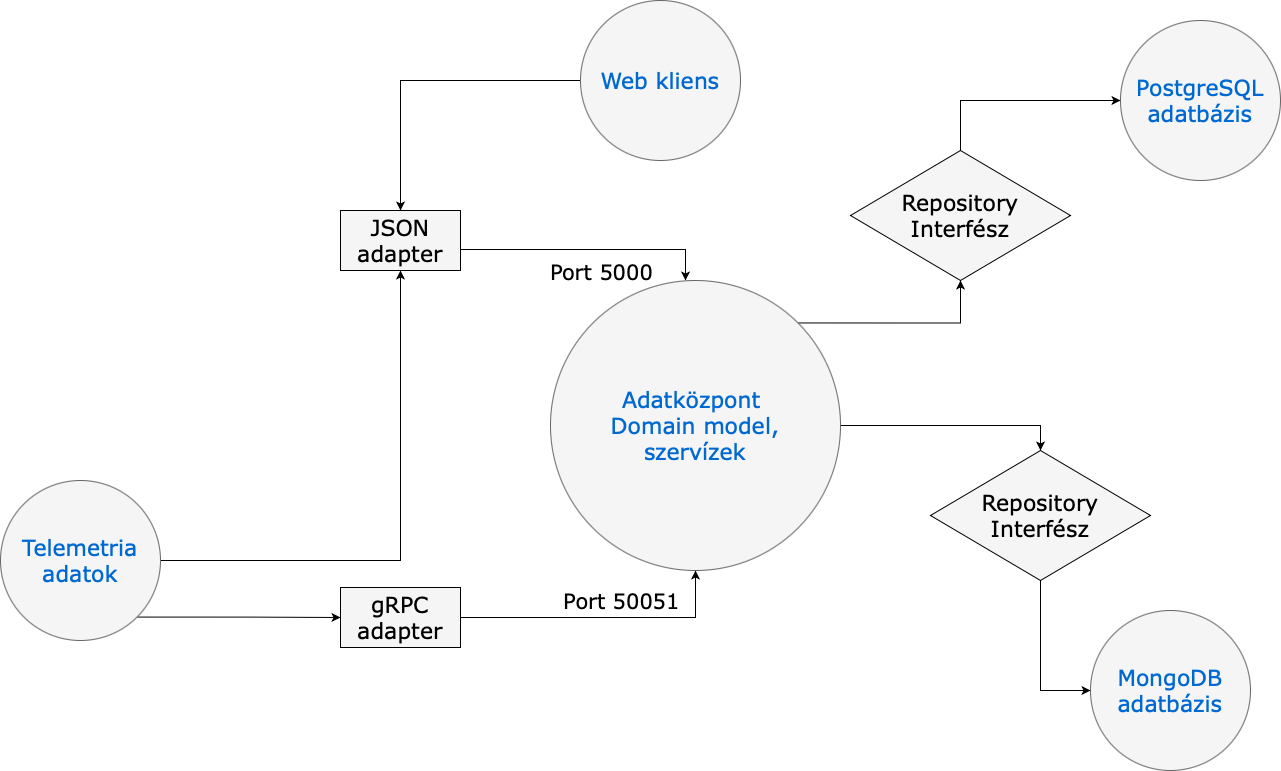
\includegraphics[scale=0.3]{images/adatkozpont-flow.png}
    \caption{Adatközpont program működésének folyamata}
    \label{fig:adatkozpont-flow}
\end{figure}

\section{A rendszer felépítése a követelmények alapján}
%TODO: ide irni Hexagonal arch. es DDD implementaciojarol. Beszurni kodot ahol latszik a repository, interface
\subsubsection{Szerkezeti felépítés}
Az alkalmazás jegyzék struktúráját a következő ábra \ref{fig:szerkezet} mutatja.
A drone-delivery jegyzék a program gyökér jegyzéke, itt található a docker-compose.yml fájl, ami az indításhoz szükséges.
A backend/server tartalmazza az adatközpont programot és a backend/drone-swarm a drón-raj programot.
Mindkét jegyzéknek hasonló a felépítése.
A cmd jegyzékbe van az indító main függvény.
A pkg jegyzék tartalmazza a kódbázis nagy részét, a domain és infrastuktúrához kapcsolódó részek itt helyezkednek el.
A pkg/domain/ben a domain kódbázis található, az infrastruktúrát és a hozzá tartozó adaptereket megvalósító kód a storage, network jegyzékekben van.
A drone-delivery/web-clientben található a web kliens, egy egyszerű html oldal ahonnan beállítjuk a szimulációt.

\begin{figure}[h]
    \centering
    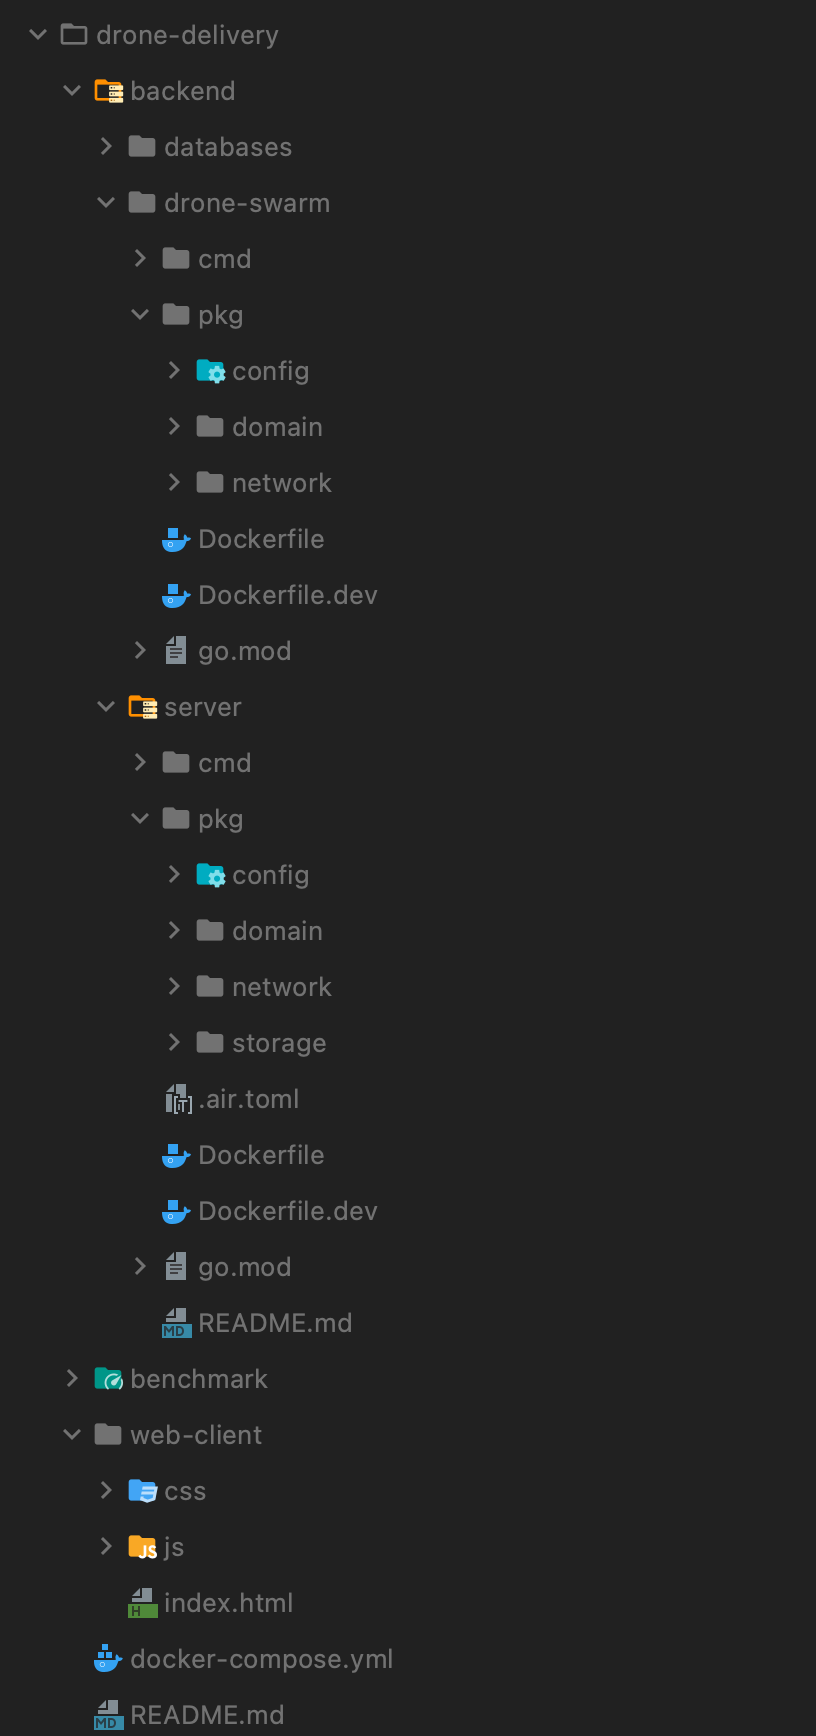
\includegraphics[scale=0.5]{images/szerkezet}
    \caption{Jegyzék szerkezet}
    \label{fig:szerkezet}
\end{figure}

\subsubsection{Portok és Adapterek, Domain Driven Design}
A hexagonal tervezési architektúra mindkét programban úgy került implementálásra, hogy a program magja, a domain üzleti logika a pkg/domain jegyzékben helyezkedik el.
Ez a domain jegyzék modellezi le az üzleti logika működését.
Itt találhatóak az interfészek, amik a hexagonal architektúra portjaiként szolgálnak, ezt kell implementálniuk az adaptereknek, így van összekötve a domain a különböző adapterekkel.
A DDD elemeit is megfigyelhetjük az elnevezésekből, valamint vannak Entity-k és Value Objectek.
\begin{python}
    # Entity
    type Drone struct {
        ID           int           `json:"id" db:"drone_id" bson:"id"`
        Telemetry    Telemetry     `json:"telemetry" bson:"telemetry"`
        Parcel       Parcel        `json:"parcel"`
        Destinations []Destination `json:"destinations"`
        Consumption  float64       `json:"consumption" db:"consumption" bson:"consumption"`
        Weight       float64       `json:"weight" db:"weight" bson:"weight"`
        State        DroneState    `db:"state" bson:"state"`
    }

    # Value Object
    type Destination struct {
        Coordinates          GPS
        ParcelDestination    bool
        WarehouseDestination bool
    }

    # Value Object
    type GPS struct {
        Latitude  float64 `json:"latitude" bson:"latitude"`
        Longitude float64 `json:"longitude" bson:"longitude"`
    }
\end{python}

\paragraph{Portok}\mbox{} \\
Minden szervízhez tartozik interface (port) amin az adapterek vagy más szervízek meghívhatják a szervíz metódusait.
Például az adatközpont drón szervízében olyan metódusok találhatóak amiket a REST API hív meg.
Itt a REST API az adapter, pontosabban vezérlő adapter.

\begin{python}
    type Service interface {
        DeliverParcels() error
        ProvisionDrone(wh models.Warehouse, d models.Drone) error
        GetFreeDrones() ([]models.Drone, error)
        GetDronesDelivering() ([]models.Drone, error)
        ChangeService(r Repository)
        ReinitializeDatabase(repos ...Repository) error
    }
\end{python}
Vezérelt adaptere az adatbázist és kimenő kommunikációt megvalósító adapterek.
Az adatközpont programban az adatbázisoknak a Repository interfészt kell implementálni, de a gRPC és JSON kommunikációhoz is tartozik interfész.
\begin{python}
    type Repository interface {
        GetFreeDrones() ([]models.Drone, error)
        GetParcelsInWarehouse() ([]models.Parcel, error)
        GetWarehouse() (models.Warehouse, error)
        GetDronesDelivering() ([]models.Drone, error)
        SetDroneState(droneID int, state string) error
        ReInitializeDeliveryData(drones []models.Drone, parcels []models.Parcel) error
    }

    type OutboundAdapter interface {
        FetchProvisionDroneEndpoint(wh models.Warehouse, d models.Drone) (success bool, err error)
    }
\end{python}

Ugyanígy a drón-raj programban.
\begin{python}
    type OutboundAdapter interface {
        SendTelemetryDataToServer(t models.Telemetry) error
    }
\end{python}
\paragraph{Adapterek} \mbox{} \\
Az adaptereket a portokon keresztül érjük el.
Alább a drón-raj program OutboundAdapter interfészét megvalósító adapter implementációját látjuk, gRPC-vel.
Csak azokat a részeket tartalmazza a példa ami szükséges a megértéshez.
Mivel a "SendTelemetryDataToServer(t models.Telemetry) error " metódus megtálható az adapterben, az interfész teljesül és az adapter használható a porton keresztül.
\begin{python}
    package grpc
    ...
    type Adapter struct {
        cc  *grpc.ClientConn
        tsc protobuf.TelemetryServiceClient
        streams map[int]StreamClient
    }

    func NewOutBoundAdapter() *Adapter {
        ...
    }

    func (a *Adapter) SendTelemetryDataToServer(t models.Telemetry) error {
        var err error
        var streamer protobuf.TelemetryService_TelemetryStreamClient
        ...
        telemetryDataRequest := protobuf.TelemetryDataRequest{
            Telemetry: &protobuf.Telemetry{
                Speed: t.Speed,
                Location: &protobuf.GPS{
                    Latitude:  t.Location.Latitude,
                    Longitude: t.Location.Longitude,
                },
                Altitude:           t.Altitude,
                Bearing:            t.Bearing,
                Acceleration:       t.Acceleration,
                BatteryLevel:       int32(t.BatteryLevel),
                BatteryTemperature: int32(t.BatteryTemperature),
                MotorTemperatures:  temperatures,
                Errors:             telemetryErrors,
                TimeStamp:          timestamppb.New(t.TimeStamp),
                DroneId:            int32(t.DroneID),
            },
        }
        err = streamer.Send(&telemetryDataRequest)
    }

\end{python}

Az adatközpont program MongoDB és PostgreSQL adatbázisához kapcsolódó, a Repository interfészt megvalósító adapterek a pkg/storage jegyzékben helyezkednek el.


\subsubsection{Dependency Injection}
A Hexagonal architektúra elvárja a kicserélhetőséget, laza kapcsolatokat és hogy az alkalmazás komponensek portokon kapcsolódjanak össze.
Ennek más előnyei is vannak, így lényegesen könnyebb a tesztelhetőség és karbantartás.
Arról már volt szó, hogy mik az adapterek és hogyan használjuk őket a portokon keresztül.
De arról még nem volt szó, hogy pontosan hogyan adjuk át az adaptereket, hogyan hivatkozunk az adapterekre.
Ehhez dependency injekciót használunk.
Azaz létrehozunk egy adaptert, szolgáltatást (szervíz) és azt átadjuk egy másik szolgáltatásnak, adapternek.
Olyan is előfordulhat, hogy a az alkalmazás domain részében két szolgáltatás egymás között portokon kommunikál.
Például a drón szolgáltatás létrehozásához szükséges paramétereket az alábbi kódrészletben láthatjuk.
Ezekből a paraméterekből a Repository, OutboundAdapter típusúak portok más adapterekhez.
Később a szolgáltatásban ezekre a portokra hivatkozunk, ezeken keresztül érjük el az adapterek metódusait.

\begin{python}
    func NewService(r Repository, ea OutboundAdapter, l gokitlog.Logger, rs routing.Service) *service {
        return &service{r, ea, l, rs}
    }
\end{python}

Az alábbi példán láthatjuk, hogy a postgreSQL, mongoDB adatbázisokat implementáló, és a külső kommunikációért felelős JSON adaptert átadjuk különböző szolgáltatásoknak.
Ezek rendre postgresStorage, mongoStorage, jsonAdapter.
\begin{python}
    postgresStorage, err := postgres.NewStorage(config.PostgresConfig)
    ...
    mongoStorage, err := mongodb.NewStorage(config.MongoConfig)
    ...
    jsonAdapter := outbound.NewJSONAdapter()
    geo := ellipsoid.Init("WGS84", ellipsoid.Degrees, ellipsoid.Meter, ellipsoid.LongitudeIsSymmetric, ellipsoid.BearingIsSymmetric)
    ...
    ts = telemetry.NewService(postgresStorage, logger, geo)
    rs = routing.NewService(logger)
    ds = drone.NewService(postgresStorage, jsonAdapter, logger, rs)
\end{python}

Majd a szolgáltásokat átadjuk egy vezérlő adapternek, egy REST API-nak ami kéréseket fogad és ez alapján a szolgáltatások portjain a megfelelő metódust meghívja.
\begin{python}
    router := rest.Handler(ds, ts, postgresStorage, mongoStorage)
\end{python}

%TODO: szekvencia diagramok is a mukodesrol, a kodban. Main fgv. -> newservice ... -> rest es grpc endpoint

\subsubsection{Konfiguráció}
A konfiguráció beállításáért a config csomag felel.
Az adatközpont, és drón-raj programban is található egy SetConfig függvény a config csomagban.
Ez környezeti változókat olvas ki, és az alapján beállítja a megfelelő értékeket.
A környezeti változókat a docker-compose.yml fájlban tudjuk módosítani.

\begin{python}
    func SetConfig() {
        flag.StringVar(&DroneSwarmURL, "drone swarm domain url", os.Getenv("DRONE_SWARM_URL"),
        "An url for the drone swarm application, with protocol")

        PostgresConfig.UserName = os.Getenv("PGUSER")
        PostgresConfig.Database = os.Getenv("PGDATABASE")
        PostgresConfig.Host = os.Getenv("PGHOST")
        PostgresConfig.Port = os.Getenv("PGPORT")
        PostgresConfig.SSSLMode = os.Getenv("PGSSL")
        PostgresConfig.PW = os.Getenv("PGPASSWORD")

        MongoConfig.UserName = os.Getenv("MONGO_USER")
        MongoConfig.Database = os.Getenv("MONGO_DB")
        MongoConfig.Host = os.Getenv("MONGO_HOST")
        MongoConfig.Port = os.Getenv("MONGO_PORT")
        MongoConfig.PW = os.Getenv("MONGO_PWD")
    }
\end{python}

\begin{python}
    func SetConfig() {
        flag.StringVar(&ServerHTTPDomain, "server domain for http", os.Getenv("SERVER_DOMAIN"), "domain of server, with protocol")
        flag.StringVar(&ServerHTTPPort, "server port for http", os.Getenv("SERVER_PORT"), "the port the server is listening on")
        flag.StringVar(&ServerGRPCDomain, "server domain for grpc", os.Getenv("SERVER_GRPC_DOMAIN"), "domain of server, with protocol")
        flag.StringVar(&ServerGRPCPort, "server port for grpc", os.Getenv("SERVER_GRPC_PORT"), "the port the server is listening on")

        PostgresConfig.UserName = os.Getenv("PGUSER")
        PostgresConfig.Database = os.Getenv("PGDATABASE")
        PostgresConfig.Host = os.Getenv("PGHOST")
        PostgresConfig.Port = os.Getenv("PGPORT")
        PostgresConfig.SSSLMode = os.Getenv("PGSSL")
        PostgresConfig.PW = os.Getenv("PGPASSWORD")
    }
\end{python}



\section{Az rendszer működése}

A rendszer úgy működik, hogy először elindul az adatközpont program, felcsatlakozik az adatbázisokra, létrejönnek a vezérelt adapterek.
Ezeket az adaptereket átadjuk a szolgáltatásoknak. Létrehozzuk a vezérlő adaptereket, ezeknek az adaptereknek átadjuk a szolgáltatásokat.
A két vezérló adapter az adatközpontban a REST API ami 5000-es porton hallgat, illetve a gRPC végpont ami 50051-es porton hallgat.
A drón raj program elindul, hasonló módon mint az adatközpont programban, először a vezérelt adapterek, majd a vezérlő adapterek jönnek létre.
Létrejön a gRPC kapcsolat az adatközpont és drón-raj program között.
A drón raj program REST API-ja a 2000-es porton hallgat.
A web klienssel indíthatjuk a szimulációt, miután megnyitottuk a böngészővel, egy egyszerű kezelő felület fogad.

A folyamat \ref{fig:mukodes} röviden úgy néz ki, hogy:
\begin{enumerate}
    \item A web kliensben kiválasztjuk, hogy milyen protokollt és formátumot, valamint adatbázist szeretnénk használni. Alapértelmezettként PostgreSQL adatbázis és HTTP/1.1 protokoll JSON formátummal van kiválasztva.
    \item A szimuláció indítása gomb megnyomásával az adatközpont program REST API \textit{/api/delivery} végpontjára küld egy POST requestet a web kliens.
    \item Az adatközpont lekérdezi a drónokat és csomagokat, majd ezek alapján optimalizálja az útvonalakat.
        A drónoknak most már megvan a hozzájuk tartozó csomagjuk és az útvonal amin haladniuk kell.
    \item Ezt az információt az adatközpont elküldi egy POST requestben a drón raj program REST API \textit{/provision} végpontjára.
    \item A drón-raj program szimulálja a drónok működését, és telemetria adatokat küld az adatközpontnak JSON vagy gRPC formátumban, attól függ mit választottunk.
    \item Az adatközpont elmenti az adatokat PostgreSQL vagy MongoDB adatbázisba, attól függ melyikbe, hogy mit választottunk.
\end{enumerate}

\begin{figure}[h]
    \centering
    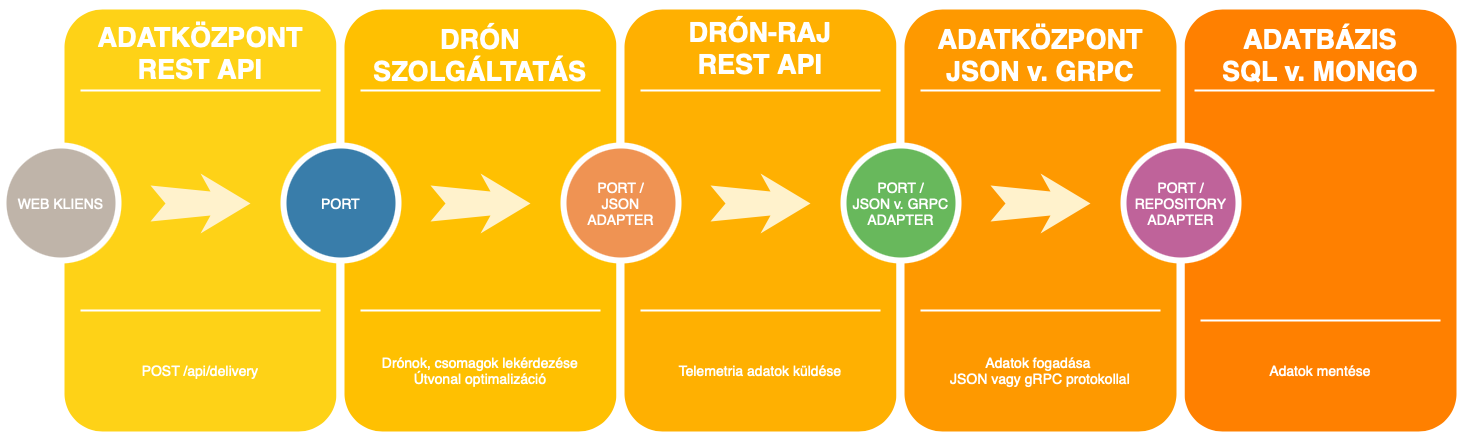
\includegraphics[scale=0.3]{images/mukodes}
    \caption{Az szimuláció folyamata}
    \label{fig:mukodes}
\end{figure}



\section{Telepítés, tesztelés}
\subsubsection{Adatbázisok elindítása}
A rendszer indítása úgy kezdődik, hogy megbizonyosodunk arról, hogy a MongoDB adatbázis és a PostgreSQL adatbázis fut és lehet rá csatlakozni.
Ha ez a 2 adatbáziskezelő nem található meg gépünkön, akkor először telepíteni kell őket.
Nálam a következőképp néz ki az indítás. A terminálban elindítom a MongoDB adatbázist.
\begin{lstlisting}[language=bash]
  $ brew services stop mongodb-community@4.4
\end{lstlisting}

Ezután a mongo parancsot kiadva kapcsolódom az adatbáziskezelő konzolos felületére.
Megbizonyosodom, hogy létezik a drone\_delivery adatbázis.
Ha nem létezik, lefuttatom a telepítéshez szükséges parancsokat \ref{subsubsec:mongodb-telepítése-az-alkalmazáshoz}.
\begin{lstlisting}[language=bash]
  $ mongo
\end{lstlisting}


Ezután elindítok egy PostgreSQL 11 vagy újabb verziójú PostgreSQL adatbázist, a fejlesztői környezetemben ez egy Postgres nevű grafikus kezelőfelületű program által történik.
Megbizonyosodok arról, hogy létezik a dbdrone\_delivery adatbázis, és létezenek a megfelelő táblák. Ha nem léteznek, lefuttatom telepítéshez szükséges scriptet \ref{subsubsec:postgresql-telepítése-a-programhoz}.

\subsubsection{Alkalmazás indítása Dockerrel}
Az alkalmazást Docker konténerben indítom el a teszteléshez, így minden fejleszői környezetében elindul, ahol van telepítve a Docker.
Az indításhoz elengedhetetlen 2 feltétel teljesülése: az adatbázisok futnak, és a \textit{docker-compose.yml} fájlban a megfelelő konfiguráció van beállítva.
A \textit{drone-delivery} jegyzékben, a terminálban kiadom a következő parancsot.
\begin{lstlisting}[language=bash]
  $ docker-compose up --build
\end{lstlisting}

\begin{figure}[h]
    \centering
    \includegraphics[scale=0.3]{images/docker-build}
    \caption{Docker build, elindulnak a programok}
    \label{fig:docker-build}
\end{figure}

Ez megépíti a konténereket, letölti a szoftver függőségeket illetve csomagokat, majd a konténerekben elindulnak a programok\ref{fig:docker-build}.
Ezután nincs más dolgunk, mint a \textit{drone-delivery/web-client} jegyzékben található \textit{index.html} fájlt megnyitni a böngészőben, az egyértelmű kezelőfelülettel tudjuk konfigurálni és indítani a szimulációt.
Egy 3D diagramon nézhetjük ahogy a drónok mozognak.
\begin{figure}[h]
    \centering
    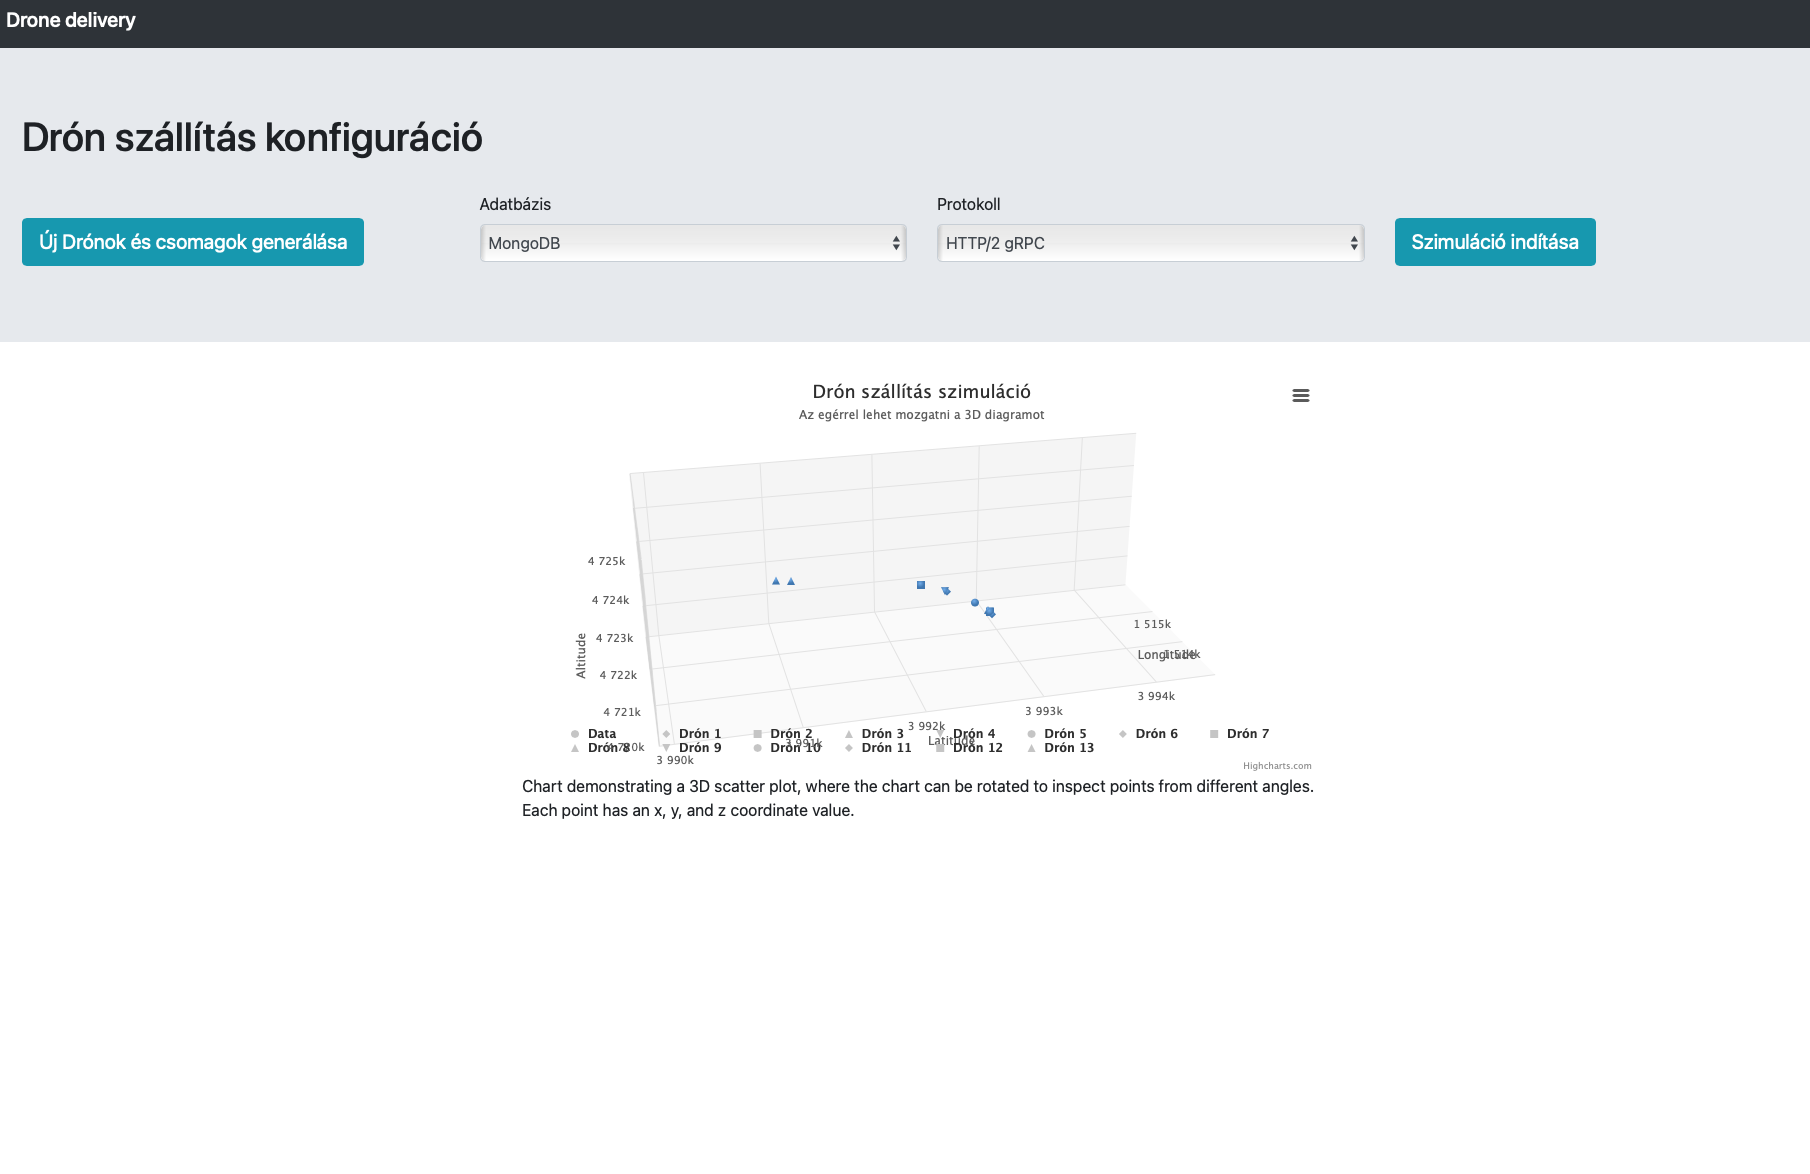
\includegraphics[scale=0.2]{images/web-client}
    \caption{Web kliens, szimuláció 3D diagramon}
    \label{fig:web-client}
\end{figure}

\section{Szállítási probléma a programban}
\subsubsection{Az adatközpont távolság számítása}
Az adatközpont program az Ortodroma számítást használja, hogy kiszámolja a távolságot a legoptimálisabb útvonal keresése közben.
\begin{python}
    func (s *service) CalculateDistance(lat1, lng1, lat2,
    lng2 float64, unit ...string) float64 {
        const PI = float64(math.Pi) //3.141592653589793

        radlat1 := PI * lat1 / 180
        radlat2 := PI * lat2 / 180

        theta := lng1 - lng2
        radtheta := PI * theta / 180

        dist := math.Sin(radlat1)*math.Sin(radlat2) +
        math.Cos(radlat1)*math.Cos(radlat2)*math.Cos(radtheta)

        if dist > 1 {
            dist = 1
        }

        dist = math.Acos(dist)
        dist = dist * 180 / PI
        dist = dist * 60 * 1.1515

        if len(unit) > 0 {
            if unit[0] == "K" {
                dist = dist * 1.609344
            } else if unit[0] == "N" {
                dist = dist * 0.8684
            } else if unit[0] == "METER" {
                dist = dist * 1.609344 * 1000
            }
        }

        return dist
    }
\end{python}
\subsubsection{A drón-raj program számításai}
A pontos szimulációs értékekhez egy könyvtárat használunk, ami megfelel a WGS84 GPS rendszernek.
Ezzel a könyvtárral pontos adatokat tudunk generálni a drón helyzetéről, irányáról.

\begin{python}
    geo := ellipsoid.Init("WGS84", ellipsoid.Degrees, ellipsoid.Meter,
    ellipsoid.LongitudeIsSymmetric, ellipsoid.BearingIsSymmetric)
    routingService := routing.NewService(geo)
\end{python}

Ezután a útvonalakért felelős szervízben két metódussal számoljuk ki a szükséges értékeket.
A \textit{CalculateDroneDistanceAndDirectionFromDestination} metódussal adott induló koordináták alapján megkapjuk a legrövidebb utat a célkoordinátákhoz, és az irányt is.
A \textit{CalculateDroneNextCoordinates} metódus megmondja adott induló koordináták és távolság valamint irány alapján hogy hova érkezünk, azaz a célkoordinátákat.

\begin{python}
    func (s *service) CalculateDroneDistanceAndDirectionFromDestination(
    currentLat, currentLon, destinationLat, destinationLon float64)
    (distance, bearing float64) {
        distance, bearing = s.geometry.To(currentLat,
        currentLon, destinationLat, destinationLon)
        return distance, bearing
    }

    func (s *service) CalculateDroneNextCoordinates(lat, lon,
    dist, bearing float64) (nextLat,nextLon float64) {
        nextLat, nextLon = s.geometry.At(lat, lon, dist, bearing)
        return nextLat, nextLon
    }
\end{python}

\Section{Mérések}

Az alkalmazással kapcsolatban méréseket is végeztem, JMeter\cite{apache}  és ghz\cite{ghz} programokat használtam.
Ezeket a méréseket fogom bemutatni és összehasonlítani.
Összehasonlításra kerülnek az alkalmazásban használt különböző protokollok, formátumok és adatbázisok.
Minden mérés a telemetria adatok küldését és mentését ábrázolja, ugyanolyan körülmények között.
Üres adatbázissal, összesen 10000 telemetria adatot küldünk, 100 szálon.
Minden egyes méréshez tartozik egy rövid összegzés, hisztogramok a teljesítményről.

\subsection{JMeter}
A Jmeteres méréshez készítettem egy \textit{telemetria.jmx}\ref{fig:jmeter-meres} konfigurációs fájlt.
A mérést úgy állítottam be, hogy 100 szálon küldünk összesen 10000 db telemetria adatot.
\begin{figure}[h]
    \centering
    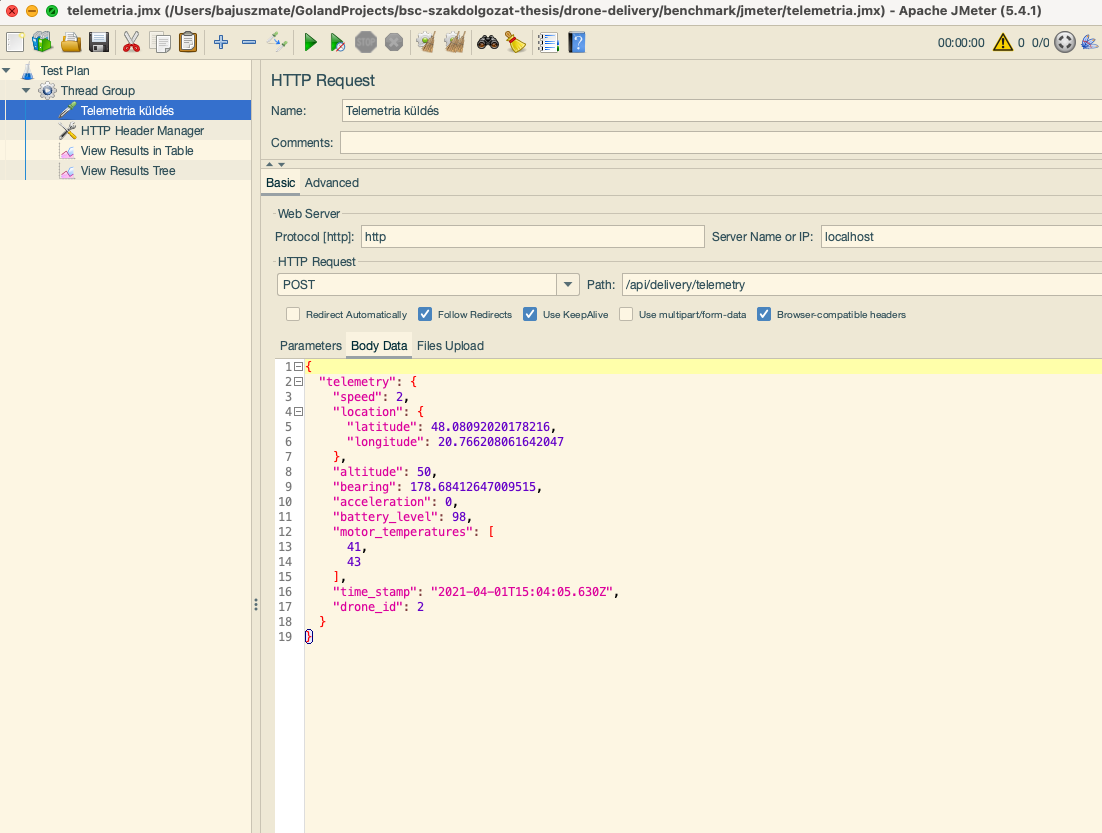
\includegraphics[scale=0.3]{images/jmeter-meres}
    \caption{Jmeter telemetria.jmx}
    \label{fig:jmeter-meres}
\end{figure}
Ez a \textit{drone-delivery/benchmark/jmeter} jegyzékben található.
A mérést úgy végeztem, hogy két jegyzékben lefuttattam a következő parancsot.
\begin{itemize}
    \item \textit{drone-delivery/benchmark/jmeter/mongo}
    \item \textit{drone-delivery/benchmark/jmeter/postgres}
\end{itemize}
\begin{lstlisting}[language=bash]
  $ jmeter -n -t ./../telemetria.jmx -l ./benchmark.csv -e -o  ./output
\end{lstlisting}

\subsubsection{HTTP/1.1 JSON, PostgreSQL adatbázissal}
\begin{figure}[hbt!]
    \centering
    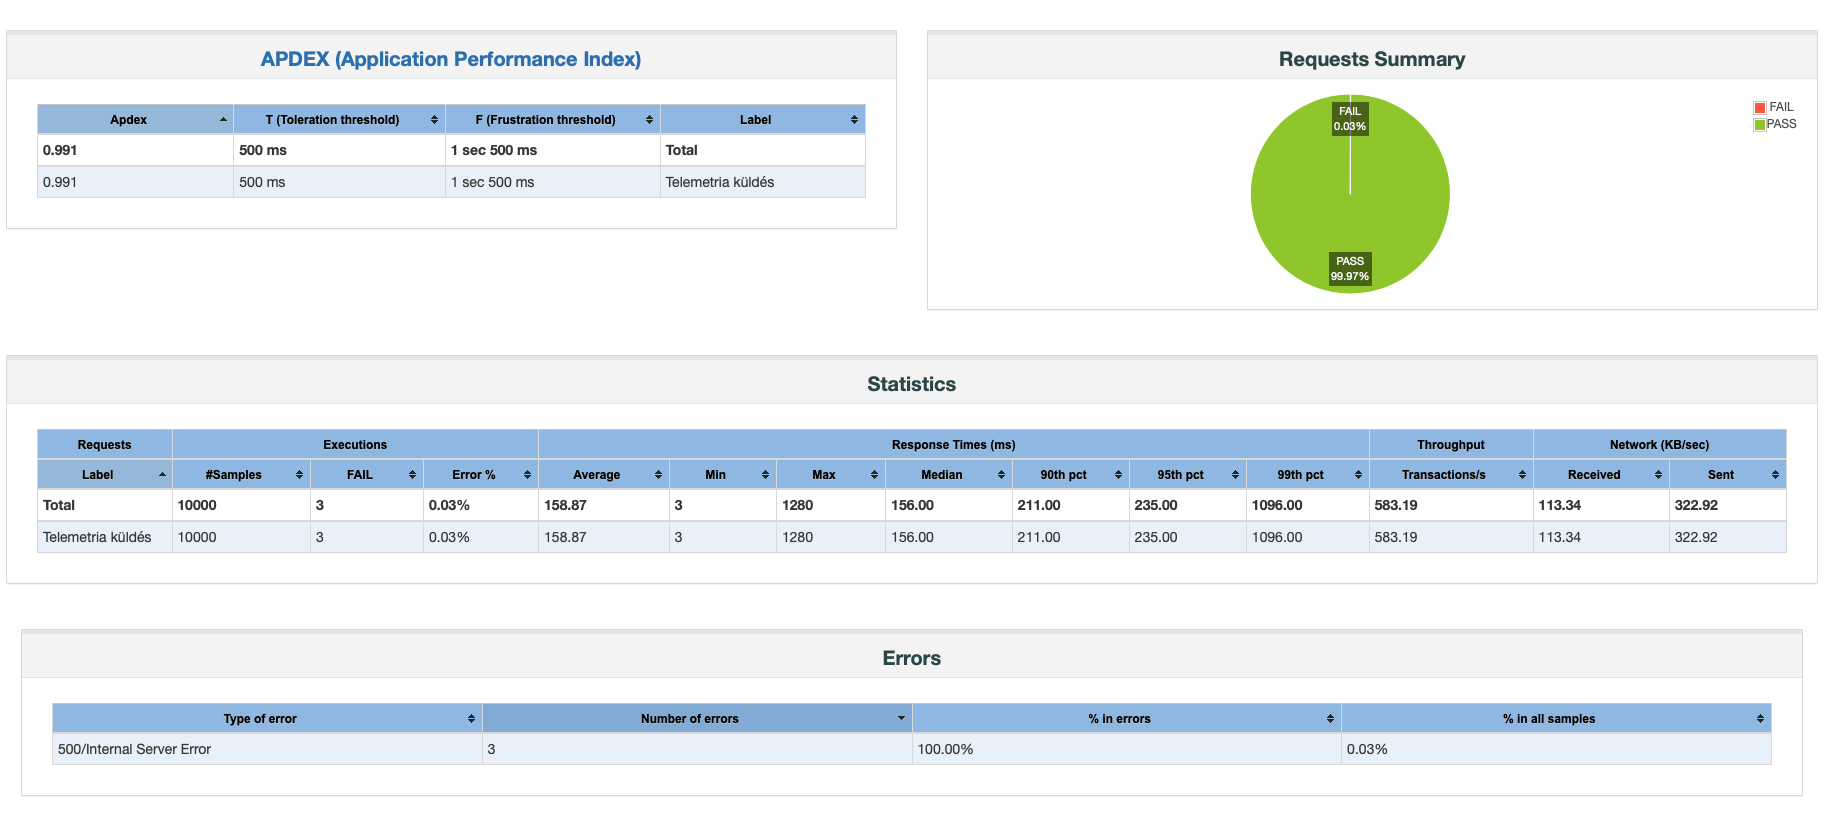
\includegraphics[scale=0.2]{images/jmeter-json-postgres}
    \caption{Jmeter mérései PostgreSQL adatbázissal HTTP/1.1 protokoll JSON formátummal}
    \label{fig:jmeter-json-postgres}
\end{figure}

\begin{figure}[hbt!]
    \centering
    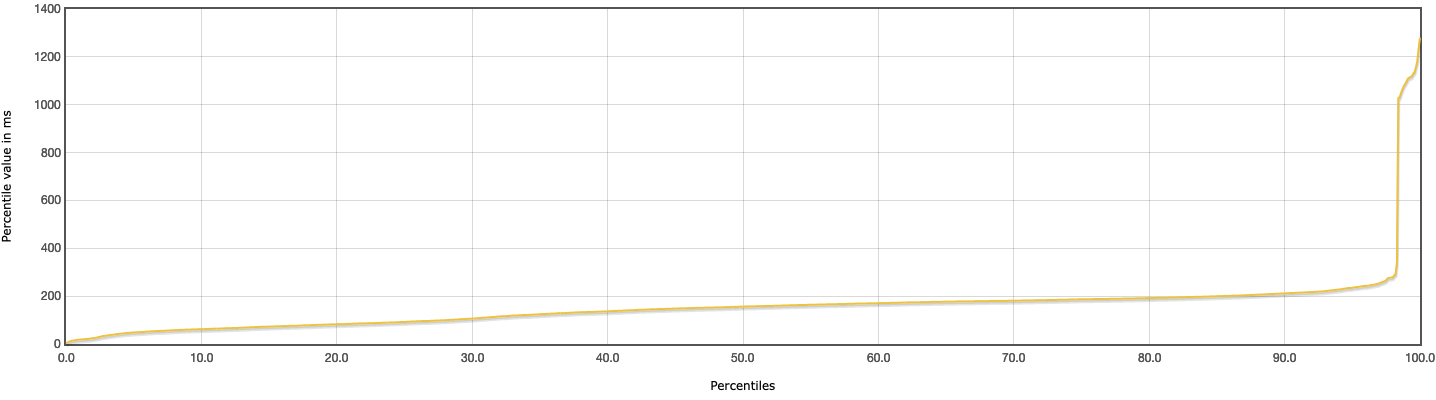
\includegraphics[scale=0.3]{images/json-postgres-response-times}
    \caption{Válaszidők PostgreSQL / JSON konfiguráció}
    \label{fig:json-postgres-response-times}
\end{figure}

\begin{figure}[hbt!]
    \centering
    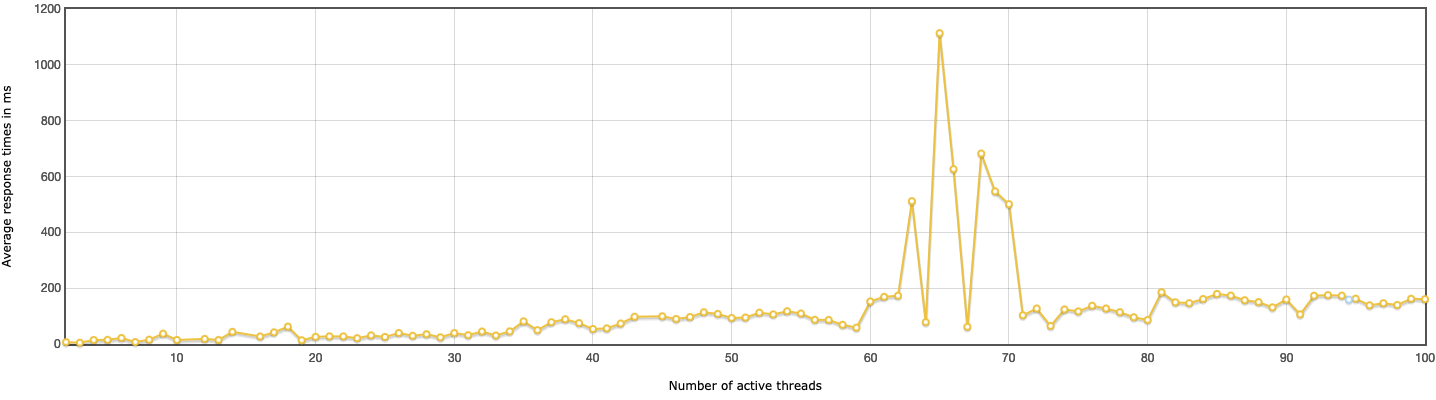
\includegraphics[scale=0.3]{images/json-time-vs-threads}
    \caption{Idő és szálak kapcsolata PostgreSQL / JSON konfiguráció}
    \label{fig:json-time-vs-threads}
\end{figure}

A mérés közben a PostgreSQL adatbázis nem tudta kezelni a túl sok kapcsolatot \ref{fig:jmeter-json-postgres}, így 3-szor hibával tért vissza a mentés.

\subsubsection{HTTP/1.1 JSON, MongoDB adatbázissal}
\begin{figure}[hbt!]
    \centering
    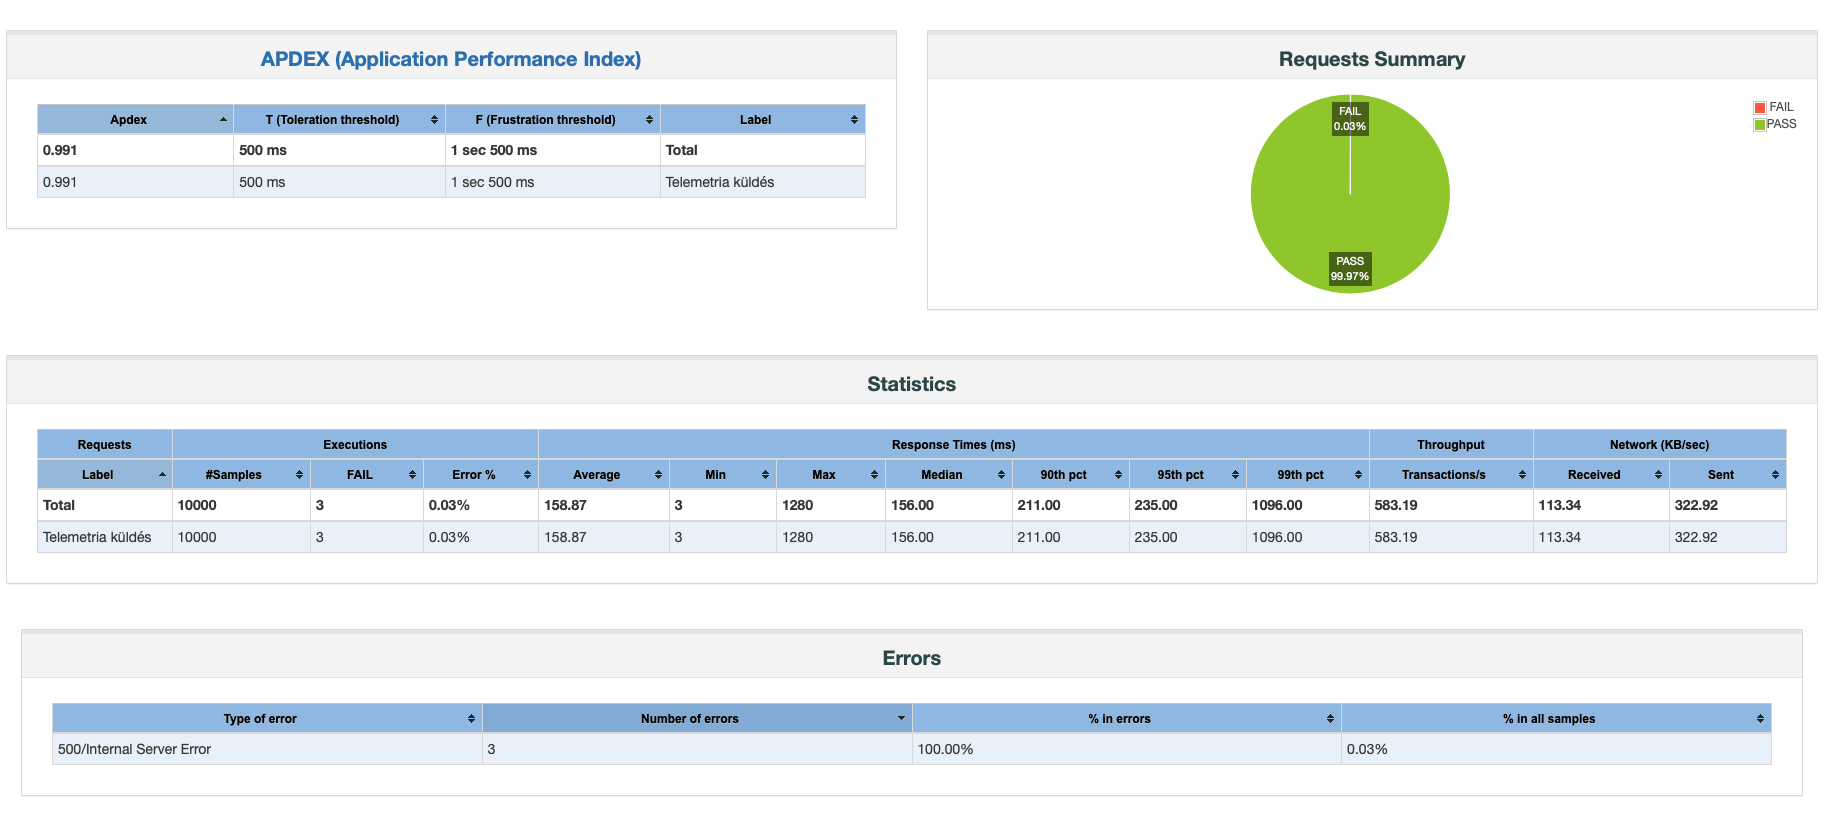
\includegraphics[scale=0.2]{images/jmeter-json-postgres}
    \caption{Jmeter mérései MongoDB adatbázissal HTTP/1.1 protokoll JSON formátummal}
    \label{fig:jmeter-json-mongo}
\end{figure}

\begin{figure}[hbt!]
    \centering
    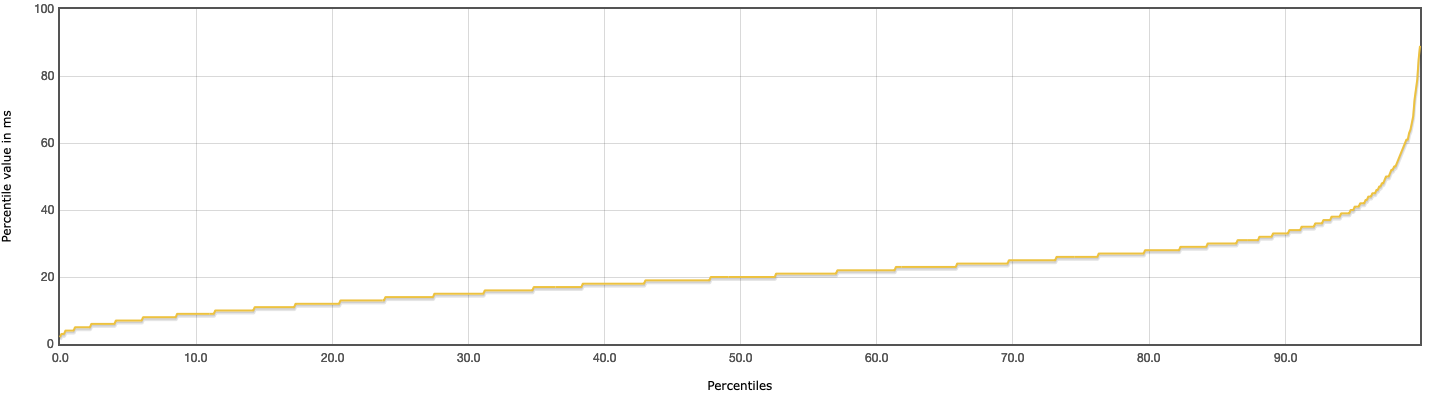
\includegraphics[scale=0.3]{images/json-mongo-response-times}
    \caption{Válaszidők MongoDB / JSON konfiguráció}
    \label{fig:json-mongo-response-times}
\end{figure}

\begin{figure}[hbt!]
    \centering
    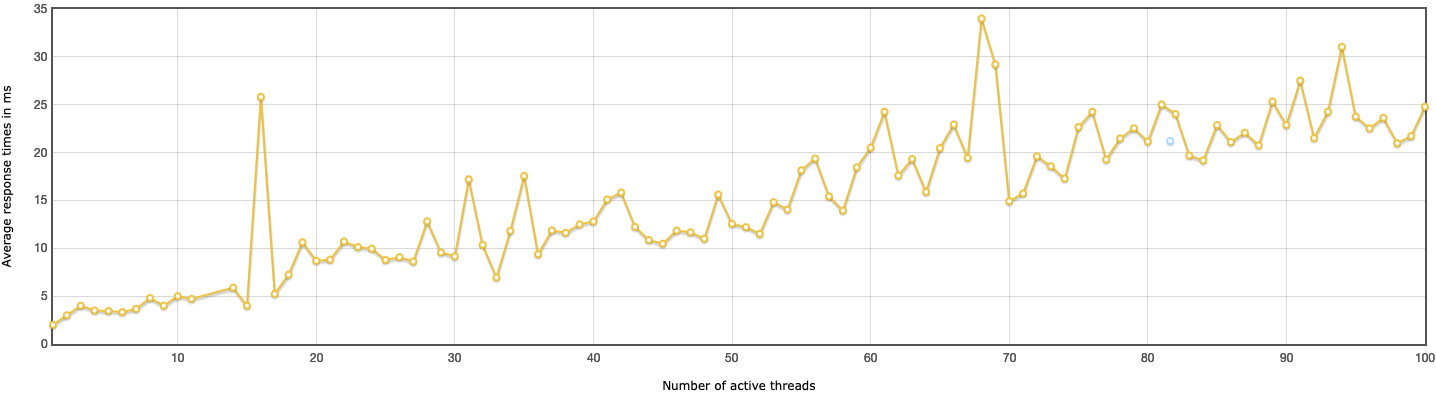
\includegraphics[scale=0.3]{images/json-mongo-time-vs-threads}
    \caption{Idő és szálak kapcsolata MongoDB / JSON konfiguráció}
    \label{fig:json-mongo-time-vs-threads}
\end{figure}
\begin{remark}
    A MongoDB adatbázis jobban teljesített mint a PostgreSQL.
    Az erőforrásokat is jobban használta ki, a mérések alapán azt a következtetést vonhatjuk le, hogy a PostgreSQL-ben sok konkurrens írás nem hatékony, a teljesítmény rovására megy.
\end{remark}

\subsection{ghz}
A ghz egy gRPC terhelés tesztelő program. Nincs hozzá grafikus felület.
Először \href{https://github.com/bojand/ghz}{feltelepítjük a ghz programot}, majd a következő paranccsal tudjuk tesztelni, a kliens oldali Telemetria streamelést az alkalmazásunkhoz.
Azaz itt a drón raj helyett a ghz program küldi a telemetria adatokat.
Az output formátumnak html-t adtam meg, a \textit{-c} paraméter a konkurrencia (szál) értéket jelöli, 100-at adtam meg.
A \textit{-n} paraméter requestek számát jelöli, ezt 10000-re állítottam.

\begin{lstlisting}[language=bash]
  $  ~ ghz -c 100 -n 10000 --format html --output report-gRPC-postgres.html  --insecure \
  --proto /Users/bajuszmate/go/src/github.com/bajusz15/ghz-benchmark/ghz/cmd/benchmark/protobuf/telemetry.proto \
  --call telemetry_grpc.TelemetryService.TelemetryStream \
  -d '[
  {
    "telemetry": {
      "speed": 2,
      "location": {
        "latitude": 48.08092020178216,
        "longitude": 20.766208061642047
      },
      "altitude": 50,
      "bearing": 178.68412647009515,
      "acceleration": 0,
      "battery_level": 98,
      "motor_temperatures": [],
      "time_stamp": "2021-04-01T15:04:05.630Z",
      "drone_id": 2
    }
  },
  {
    "telemetry": {
      "speed": 2,
      "location": {
        "latitude": 48.08092020178216,
        "longitude": 20.766208061642047
      },
      "altitude": 50,
      "bearing": 178.68412647009515,
      "acceleration": 0,
      "battery_level": 98,
      "motor_temperatures": [],
      "time_stamp": "2021-04-01T15:04:05.630Z",
      "drone_id": 2
    }
  }
]' \
  localhost:50051
\end{lstlisting}

\subsubsection{HTTP/2 gRPC, PostgreSQL adatbázissal \ref{fig:ghz-postgres}}

\begin{figure}[hbt!]
    \centering
    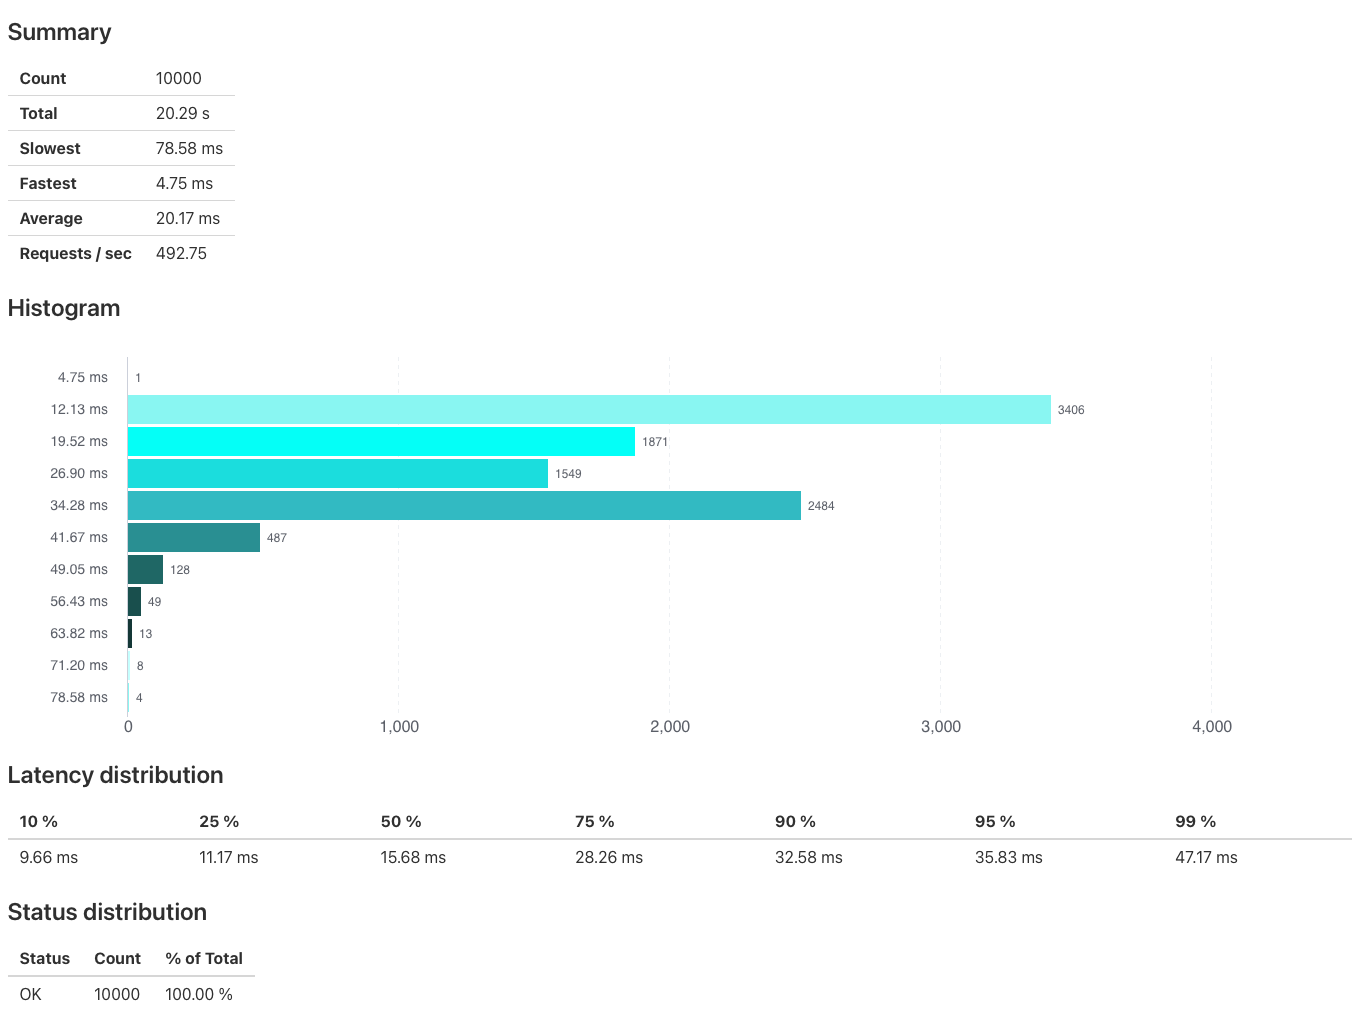
\includegraphics[scale=0.3]{images/ghz-postgres}
    \caption{Ghz mérései PostgreSQL adatbázison, gRPC}
    \label{fig:ghz-postgres}
\end{figure}

\begin{remark}
    A gRPC sokkal jobban teljesített mint a JSON.
    Ezt a diagramon is láthatjuk.
    Tehát a következtetéseink jók voltak, a HTTP/2 gRPC sokkal hatékonyabb mint a HTTP/1.1 JSON.
\end{remark}


\subsubsection{HTTP/2 gRPC, MongoDB adatbázissal \ref{fig:ghz-mongo}}
\begin{figure}[hbt!]
    \centering
    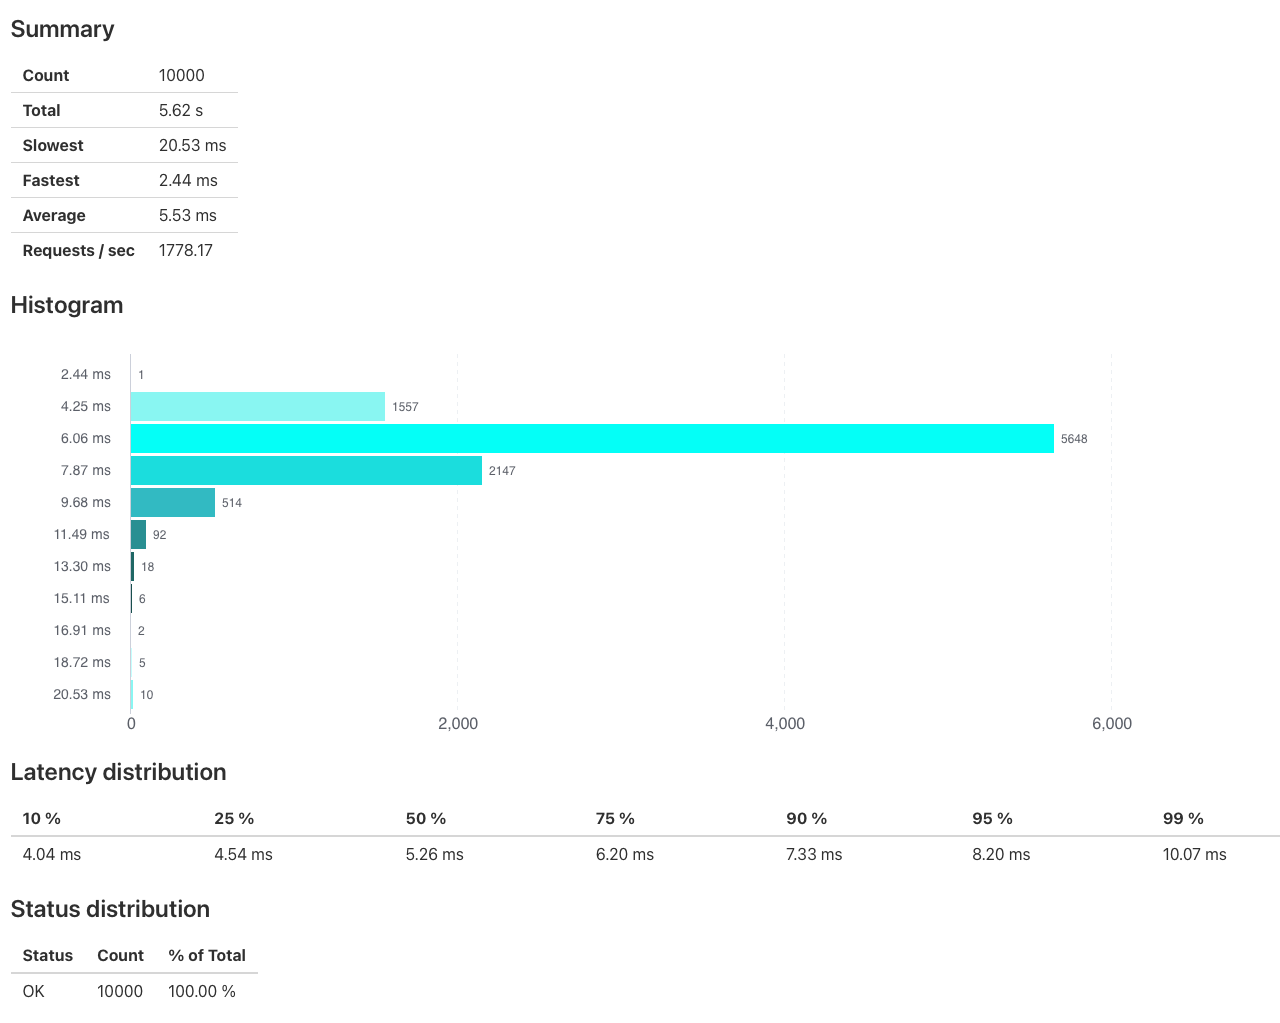
\includegraphics[scale=0.3]{images/ghz-mongo}
    \caption{Ghz mérései MongoDB adatbázison, gRPC}
    \label{fig:ghz-mongo}
\end{figure}

Összességében elmondható, hogy a gRPC a gyorsabb protokoll, és a MongoDB hatékonyabb erre a feladatra mint a PostgreSQL.




\Chapter{Szimuláció}

\Chapter{Tesztelés}

A fejezetben be kell mutatni, hogy az elkészült alkalmazás hogyan használható.
(Az, hogy hogyan kell, hogy működjön, és hogy hogy lett elkészítve, az előző fejezetekben már megtörtént.)

Jellemzően az alábbi dolgok kerülhetnek ide.
\begin{itemize}
\item Tesztfuttatások. Le lehet írni a futási időket, memória és tárigényt.
\item Felhasználói kézikönyv jellegű leírás. Kifejezetten a végfelhasználó szempontjából lehet azt bemutatni, hogy mit hogy lehet majd használni.
\item Kutatás kapcsán ide főként táblázatok, görbék és egyéb részletes összesítések kerülhetnek.
\end{itemize}

\Chapter{Összefoglalás}

Összességében meg vagyok elégedve az eredményekkel.
A rendszer moduláris felépítése jól sikerült, az összehasonlítások tökéletesen működtek és érdekes eredményeket produkáltak, de persze semmi meglepő nincs az eredményekben.
Számomra nagyon érdekesek a különböző architektúrák, új kommmunikációs protokollok és adatbázisok által nyújtott előnyök.
Amit hiányolok a programból, de sajnos nem maradt idő az implementálásra az egy valós idejű Apache Kafka adatcsatorna.
Az Apache Kafka egyfajta üzenet bróker, amely képes nagy forgalmú hiba toleráns működésre.
Mivel a telemetria adatokra tekinthetünk úgy mint kritikus adatok, egy ilyen modullal ki lehetne egészíteni a programot.
A drónok szimulációja lehetett volna érdekesebb, ha tudunk valós térképek alapján útvonalakat optimalizálni.
A rendszer jövőjét mindenképpen abban látom, hogy több protokollt és adatbázist lehet összehasonlítani.
Érdekes eredmények születhetnének MQTT protokollal, és más dokumentum alapú vagy nagyon sok írásra tervezett adatbázisokkal.



\clearpage

\addcontentsline{toc}{chapter}{Irodalomjegyzék}
\bibliographystyle{plain}
\bibliography{dolgozat.bib}

\newpage

\pagestyle{empty}

\noindent \textbf{\Large CD Használati útmutató}

\vskip 1cm

Ennek a címe lehet például \textit{A mellékelt CD tartalma} vagy \textit{Adathordozó használati útmutató} is.

Ez jellemzően csak egy fél-egy oldalas leírás.
Arra szolgál, hogy ha valaki kézhez kapja a szakdolgozathoz tartozó CD-t, akkor tudja, hogy mi hol van rajta.
Jellemzően elég csak felsorolni, hogy milyen jegyzékek vannak, és azokban mi található.
Az elkészített programok telepítéséhez, futtatásához tartozó instrukciók kerülhetnek ide.

A CD lemezre mindenképpen rá kell tenni
\begin{itemize}
\item a dolgozatot egy \texttt{dolgozat.pdf} fájl formájában,
\item a LaTeX forráskódját a dolgozatnak,
\item az elkészített programot, fontosabb futási eredményeket (például ha kép a kimenet),
\item egy útmutatót a CD használatához (ami lehet ez a fejezet külön PDF-be vagy MarkDown fájlként kimentve).
\end{itemize}


\end{document}
